\documentclass[10pt, aspectratio=169, xcolor=dvipsnames]{beamer}

% ---------------------------------------------------
% Packages for Rigorous Mathematics & Graphics
% ---------------------------------------------------
\usepackage[T1]{fontenc}
\usepackage{amsmath}
\usepackage{amssymb}
\usepackage{amsthm}
\usepackage{mathtools}
\usepackage{mathrsfs}
\usepackage{bm}
\usepackage{lmodern}   % High-quality vector fonts
\usepackage{tikz}
\usepackage{etoolbox}
\usepackage{svg}       % Required for SVG images (compile with --shell-escape)

% Tighter display-math spacing so formula-heavy 16:9 slides fit comfortably
\apptocmd{\normalsize}{%
  \setlength\abovedisplayskip{3pt plus 1pt minus 2pt}%
  \setlength\belowdisplayskip{3pt plus 1pt minus 2pt}%
  \setlength\abovedisplayshortskip{0pt plus 1pt}%
  \setlength\belowdisplayshortskip{2pt plus 1pt}}{}{}

% ---------------------------------------------------
% Palette
% ---------------------------------------------------
\definecolor{UniBlue}{RGB}{0, 101, 189}   % University of Luxembourg blue (approx.)
\definecolor{Navy}{RGB}{10, 31, 68}
\definecolor{Sky}{RGB}{233, 242, 251}
\definecolor{Amber}{RGB}{240, 154, 62}
\definecolor{Teal}{RGB}{23, 150, 140}
\definecolor{Slate}{RGB}{45, 55, 72}
\definecolor{Mist}{RGB}{247, 249, 252}

% ---------------------------------------------------
% Theme: a clean, custom look (no stock outer theme)
% ---------------------------------------------------
\usetheme{default}
\usefonttheme{professionalfonts}          % keep LaTeX math fonts
\setbeamertemplate{navigation symbols}{}
\setbeamersize{text margin left=1.2cm, text margin right=1.2cm}

\setbeamercolor{normal text}{fg=Slate, bg=white}
\setbeamercolor{structure}{fg=UniBlue}
\setbeamercolor{alerted text}{fg=Amber!90!black}
\setbeamercolor{item}{fg=Amber}
\setbeamercolor{footline}{fg=Slate!70, bg=white}

\setbeamerfont{frametitle}{size=\Large, series=\bfseries}

% --- Bullets ---
\setbeamertemplate{itemize item}{\raisebox{0.1ex}{\scriptsize$\blacksquare$}}
\setbeamertemplate{itemize subitem}{\raisebox{0.1ex}{\tiny$\blacktriangleright$}}

% --- Frame title: left-aligned, tri-colour underline ---
\setbeamertemplate{frametitle}{%
  \vskip 3.5mm
  {\usebeamerfont{frametitle}\color{Navy}\insertframetitle\par}
  \vskip 1.2mm
  
\begin{tikzpicture}
    \fill[UniBlue]    (0,0)   rectangle (1.8,0.07);
    \fill[Amber]      (1.8,0) rectangle (2.3,0.07);
    \fill[UniBlue!14] (2.3,0) rectangle (\linewidth,0.07);
  \end{tikzpicture}
  \vskip 1mm
}

% --- Footline: progress bar + author / title / page ---
\setbeamertemplate{footline}{%
  \leavevmode%
  \hbox to\paperwidth{%
    \color{UniBlue}\vrule height 2.4pt depth 0pt
      width \dimexpr\paperwidth*\insertframenumber/\inserttotalframenumber\relax
    \color{UniBlue!12}\leaders\hrule height 2.4pt depth 0pt\hfill}%
  \vskip 0pt%
  \hbox to\paperwidth{%
    \hskip 1.2cm%
    \color{Slate!75}\scriptsize
    \insertshortauthor\hfill\insertshorttitle\hfill%
    {\color{UniBlue}\bfseries\insertframenumber}\,/\,\inserttotalframenumber%
    \hskip 1.2cm}%
  \vskip 2.2mm%
}

% --- Blocks: soft rounded cards (theorem = blue, definition = teal) ---
\setbeamertemplate{blocks}[rounded][shadow=false]
\setbeamercolor{block title}{fg=white, bg=UniBlue}
\setbeamercolor{block body}{fg=Slate, bg=Sky}
\setbeamercolor{block title example}{fg=white, bg=Teal}
\setbeamercolor{block body example}{fg=Slate, bg=Teal!8}
\setbeamercolor{block title alerted}{fg=white, bg=Amber!90!black}
\setbeamercolor{block body alerted}{fg=Slate, bg=Amber!10}
\setbeamerfont{block title}{series=\bfseries, size=\small}

% Small coloured lead-in for run-in headings
\newcommand{\lead}[1]{{\color{UniBlue}\bfseries #1}}

% ---------------------------------------------------
% Title Page Information
% ---------------------------------------------------
\title[Two-Sided Hypothesis Testing]{Two-Sided Hypothesis Testing}
\subtitle{Sections 3.6--3.7 of \textit{Testing Statistical Hypotheses}\\
          (Lehmann \& Romano, 2022)}
\author[Jha Abhishek]{Abhishek Jha}
\institute[Uni.lu]{M.Sc.\ Mathematics \\ University of Luxembourg \\ Course MNO 0.020}
\date[Nov 24, 2026]{November 24, 2026}

% --- Custom title page (light, drawn with TikZ) ---
% NOTE: needs logo.svg in the same folder and compilation with --shell-escape.
\setbeamertemplate{title page}{%
  \begin{tikzpicture}[remember picture, overlay]
   \begin{scope}[shift={(current page.south west)}]

    % ---------- Background: soft gradient + graph paper ----------
    \begin{scope}
      \clip (0,0) rectangle (\paperwidth,\paperheight);
      \shade[top color=white, bottom color=Sky!80] (0,0) rectangle (\paperwidth,\paperheight);
      \draw[step=0.5cm, UniBlue!12, line width=0.25pt] (0,0) grid (\paperwidth,\paperheight);
      \draw[step=2.5cm, UniBlue!20, line width=0.4pt] (0,0) grid (\paperwidth,\paperheight);
      \fill[UniBlue!7] (\paperwidth,\paperheight) circle (4.8cm);

      % ---------- Compass drawing an arc (lower right) ----------
      \begin{scope}[shift={(12.0,1.05)}]
        \coordinate (A) at (0,0);        % needle point
        \coordinate (B) at (1.84,0);     % pencil point
        \coordinate (H) at (0.92,2.8);   % hinge
        % guide circles around the needle point
        \draw[UniBlue!25, line width=0.5pt] (A) circle (0.92cm);
        \draw[UniBlue!25, line width=0.5pt] (A) circle (2.76cm);
        % arc traced by the pencil
        \draw[UniBlue!70, dash pattern=on 4pt off 3pt, line width=1pt]
              (B) arc[start angle=0, end angle=118, radius=1.84cm];
        \fill[UniBlue!70] (A) circle (1.6pt);
        % legs
        \draw[Navy!85, line width=2pt, line cap=round] (A) -- (H);
        \draw[Navy!85, line width=2pt, line cap=round] (B) -- (H);
        \draw[Navy, line width=1pt, line cap=round] (A) -- ++(-0.04,-0.1);   % needle
        \draw[Amber, line width=2.8pt, line cap=round] (B) -- ++(-0.09,0.27); % pencil
        % hinge and handle
        \draw[Navy!85, line width=2pt, line cap=round] (H) -- ++(0,0.4);
        \fill[Navy] ([yshift=0.45cm]H) circle (0.1cm);
        \fill[Navy] (H) circle (0.13cm);
        \fill[white] (H) circle (0.045cm);
      \end{scope}

      % ---------- Faint theorems in the background ----------
      \begin{scope}[UniBlue, opacity=0.17, font=\sffamily]
        \node[rotate=4, font=\Large] at (8.2,7.35)
          {$\displaystyle \phi(x)=\begin{cases}1 & p_1>kp_0\\ \gamma & p_1=kp_0\\ 0 & p_1<kp_0\end{cases}$};
        \node[rotate=-4, font=\large] at (8.7,3.1)
          {$\beta_\phi(\theta)=E_\theta[\phi(X)]=\displaystyle\int\phi\,dP_\theta$};
        \node[rotate=3, font=\large] at (8.0,1.55)
          {$\displaystyle\sup_{\theta\in H}\beta_\phi(\theta)\le\alpha,\qquad \Omega=H\cup K$};
        \node[rotate=-6, font=\large] at (2.3,6.6)
          {$\displaystyle\int\phi\,p_0\,d\mu=\alpha$};
        \node[text width=5.2cm, align=justify, font=\scriptsize\itshape, rotate=2] at (13.2,6.95)
          {\textbf{Theorem.} For every level $\alpha$ there is a most powerful test of
           likelihood-ratio form. \hfill$\blacksquare$};
      \end{scope}
    \end{scope}

    % ---------- Ruler along the bottom edge ----------
    \fill[Amber!22] (0,0) rectangle (\paperwidth,0.62);
    \draw[Amber!70!black, line width=0.6pt] (0,0.62) -- (\paperwidth,0.62);
    \foreach \i in {0,...,160}{
      \pgfmathtruncatemacro{\r}{mod(\i,10)}
      \pgfmathtruncatemacro{\c}{\i/10}
      \ifnum\r=0
        \draw[Amber!70!black, line width=0.5pt] (\i/10,0.62) -- (\i/10,0.30);
        \ifnum\i<160
          \node[anchor=north, inner sep=1pt, font=\tiny\sffamily, text=Amber!60!black]
            at (\i/10+0.02,0.29) {\c};
        \fi
      \else
        \ifnum\r=5
          \draw[Amber!70!black, line width=0.4pt] (\i/10,0.62) -- (\i/10,0.40);
        \else
          \draw[Amber!70!black, line width=0.3pt] (\i/10,0.62) -- (\i/10,0.50);
        \fi
      \fi
    }

    % ---------- Logo and top label ----------
    \node[anchor=north west, inner sep=0pt] at (1.4,8.35)
      {\includesvg[width=3.5cm]{logo.svg}};
    \node[anchor=north east, text=Slate!75, font=\scriptsize\bfseries\sffamily]
      at (\paperwidth-1.4cm,8.35)
      {M.Sc.\ MATHEMATICS \;\textbullet\; COURSE MNO 0.020};

    % ---------- Title block ----------
    \node[anchor=south west, text=Navy, text width=0.86\paperwidth, align=left,
          font=\fontsize{24}{28}\selectfont\bfseries\sffamily]
      (ttl) at (1.5,4.9) {\inserttitle};
    \fill[Amber] ([yshift=-0.35cm]ttl.south west) rectangle
                 ([shift={(2.2cm,-0.43cm)}]ttl.south west);
    \node[anchor=north west, text=Slate, text width=0.68\paperwidth, align=left,
          font=\normalsize\sffamily]
      at ([yshift=-0.75cm]ttl.south west) {\insertsubtitle};

    % ---------- Author block ----------
    \node[anchor=south west, text=Navy, align=left, font=\sffamily]
      at (1.5,1.05)
      {{\large\bfseries\insertauthor}\\[3pt]
       \footnotesize\color{Slate!75}University of Luxembourg\\
       \footnotesize\color{Slate!75}\insertdate};

   \end{scope}
  \end{tikzpicture}%
}

\begin{document}

% --- Slide 1: Title Slide ---
\begin{frame}[plain]
    \titlepage
\end{frame}

% --- Slide 2: The Statistical Hypothesis Testing Framework ---
\begin{frame}{The Statistical Hypothesis Testing Framework}
    
    \vspace{0.2cm}
    \begin{center}
    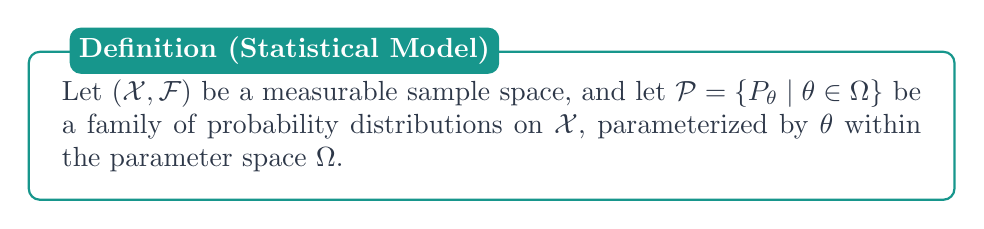
\begin{tikzpicture}
        \node[draw=Teal, thick, rounded corners, inner xsep=12pt, inner ysep=10pt, fill=white] (box1) {
            \begin{minipage}{0.9\textwidth}
                \color{Slate}
                Let $(\mathcal{X}, \mathcal{F})$ be a measurable sample space, and let $\mathcal{P} = \{P_\theta \mid \theta \in \Omega\}$ be a family of probability distributions on $\mathcal{X}$, parameterized by $\theta$ within the parameter space $\Omega$.
            \end{minipage}
        };
        \node[fill=Teal, text=white, rounded corners, right=15pt] at (box1.north west) {\bfseries Definition (Statistical Model)};
    \end{tikzpicture}
    \end{center}

    \vspace{0.2cm}
    We partition the parameter space into two disjoint subsets, $\Omega = H \cup K$ with $H \cap K = \emptyset$:
    \vspace{0.1cm}
    \begin{itemize}
        \item[{ \tikz\fill[Teal] (0,0) circle (2pt); }] \textbf{Null Hypothesis} ($H$): The default model state ($\theta \in H$).
        \vspace{0.1cm}
        \item[{ \tikz\fill[Teal] (0,0) circle (2pt); }] \textbf{Alternative Hypothesis} ($K$): The theoretical discovery ($\theta \in K$).
    \end{itemize}

    \vspace{0.3cm}
    \begin{center}
    
\begin{tikzpicture}
        \node[draw=Teal, thick, rounded corners, inner xsep=12pt, inner ysep=10pt, fill=white] (box2) {
            \begin{minipage}{0.9\textwidth}
                \color{Slate}
                A randomized test is a measurable function $\phi: \mathcal{X} \to [0,1]$ that maps the observed data $x \in \mathcal{X}$ to the probability of rejecting the null hypothesis $H$.
            \end{minipage}
        };
        \node[fill=Teal, text=white, rounded corners, right=15pt] at (box2.north west) {\bfseries Definition (Critical Function)};
    \end{tikzpicture}
    \end{center}
\end{frame}

% --- Slide 3: The Power Function and Error Control ---
\begin{frame}{Errors and the Power Function}
    
    \vspace{0.1cm}
    \begin{center}
    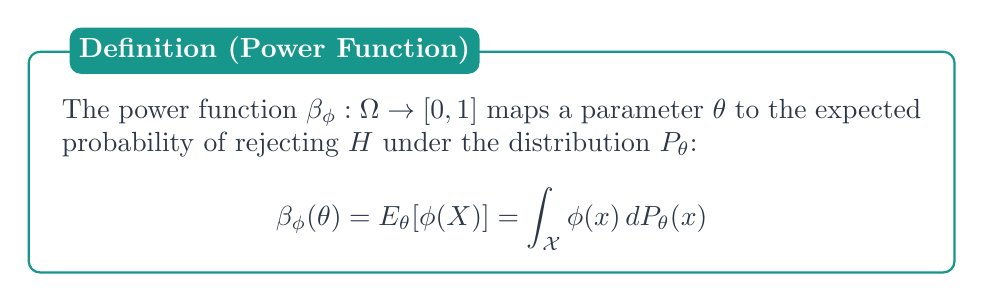
\begin{tikzpicture}
        \node[draw=Teal, thick, rounded corners, inner xsep=12pt, inner ysep=8pt, fill=white] (box1) {
            \begin{minipage}{0.9\textwidth}
                \vspace*{0.3cm} % <-- FIX: Pushes text down to clear the title banner
                \color{Slate}
                The power function $\beta_\phi: \Omega \to [0,1]$ maps a parameter $\theta$ to the expected probability of rejecting $H$ under the distribution $P_\theta$:
                \[ \beta_\phi(\theta) = E_\theta[\phi(X)] = \int_{\mathcal{X}} \phi(x) \, dP_\theta(x) \]
            \end{minipage}
        };
        \node[fill=Teal, text=white, rounded corners, right=15pt] at (box1.north west) {\bfseries Definition (Power Function)};
    \end{tikzpicture}
    \end{center}

    \vspace{0cm}
    The framework imposes a strict asymmetry on decision errors:
    
    \vspace{0.2cm}
    \begin{itemize}
        \item[{ \tikz\fill[Teal] (0,0) circle (2pt); }] \lead{Size / Level $\alpha$ (Type I Error Control):} We strictly bound the probability of falsely rejecting $H$. A test has level $\alpha$ if $\sup_{\theta \in H} \beta_\phi(\theta) \le \alpha$.
        
        \vspace{0.2cm}
        \item[{ \tikz\fill[Teal] (0,0) circle (2pt); }] \lead{Power (Avoiding Type II Error):} Subject to the level $\alpha$ constraint, we seek to maximize the probability of correctly rejecting $H$ when it is false. Our goal is to maximize $\beta_\phi(\theta)$ for all $\theta \in K$.
    \end{itemize}
\end{frame}

% --- Slide 4: Uniformly Most Powerful (UMP) Tests (Part 1) ---
\begin{frame}{Uniformly Most Powerful (UMP) Tests (1/2)}
    
    When the alternative $K$ is composite, the optimal test must dominate across all of $K$.

    \vspace{0.4cm}
    \begin{center}
    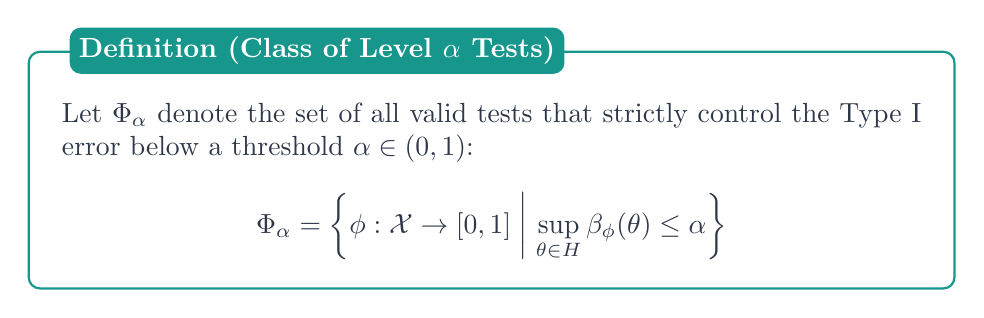
\begin{tikzpicture}
        \node[draw=Teal, thick, rounded corners, inner xsep=12pt, inner ysep=10pt, fill=white] (box1) {
            \begin{minipage}{0.9\textwidth}
                \vspace*{0.3cm} 
                \color{Slate}
                Let $\Phi_\alpha$ denote the set of all valid tests that strictly control the Type I error below a threshold $\alpha \in (0,1)$:
                \[
                    \Phi_\alpha = \left\{ \phi : \mathcal{X} \to [0,1] \;\middle|\; \sup_{\theta \in H} \beta_\phi(\theta) \le \alpha \right\}
                \]
            \end{minipage}
        };
        \node[fill=Teal, text=white, rounded corners, right=15pt] at (box1.north west) {\bfseries Definition (Class of Level $\alpha$ Tests)};
    \end{tikzpicture}
    \end{center}
\end{frame}

% --- Slide 5: Uniformly Most Powerful (UMP) Tests (Part 2) ---
\begin{frame}{Uniformly Most Powerful (UMP) Tests (2/2)}
    
    \vspace{0.2cm}
    \begin{center}
    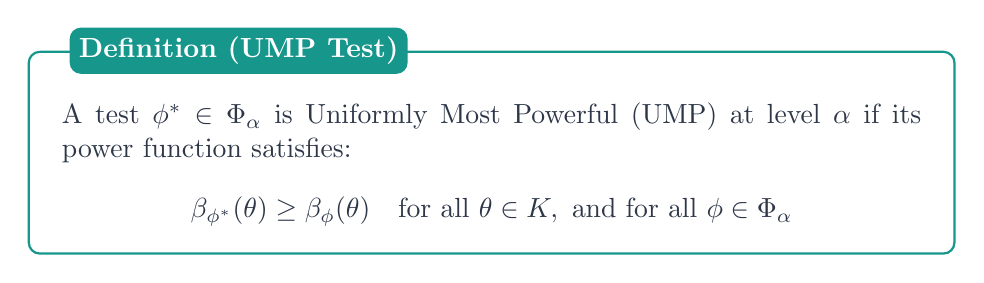
\begin{tikzpicture}
        \node[draw=Teal, thick, rounded corners, inner xsep=12pt, inner ysep=10pt, fill=white] (box2) {
            \begin{minipage}{0.9\textwidth}
                \vspace*{0.3cm} 
                \color{Slate}
                A test $\phi^* \in \Phi_\alpha$ is \alert{Uniformly Most Powerful (UMP)} at level $\alpha$ if its power function satisfies:
                \[
                    \beta_{\phi^*}(\theta) \ge \beta_\phi(\theta) \quad \text{for all } \theta \in K, \text{ and for all } \phi \in \Phi_\alpha
                \]
            \end{minipage}
        };
        \node[fill=Teal, text=white, rounded corners, right=15pt] at (box2.north west) {\bfseries Definition (UMP Test)};
    \end{tikzpicture}
    \end{center}

    \vspace{0.6cm}
    \textit{Goal:} A single test $\phi^*$ that maximizes $\beta_\phi(\theta)$ everywhere in $K$, while strictly obeying the size limit $\alpha$ in $H$.
\end{frame}

% --- Slide 5: The Neyman-Pearson Fundamental Lemma (1/2) ---
\begin{frame}{The Neyman--Pearson Fundamental Lemma (1/2)}
    
    \lead{Theorem (NP Lemma: Existence and Structure)}\\
    \vspace{0.2cm}

    \noindent
    {\color{Teal}\vrule width 4pt}%
    \hspace{10pt}%
    \begin{minipage}{\dimexpr\textwidth-14pt\relax}
        \color{Slate}
        Let $X \in \mathcal{X}$ be a random variable with probability density function (pdf) $p(x)$ with respect to a measure $\mu$. Consider testing the simple null hypothesis $H: p = p_0$ versus the simple alternative $K: p = p_1$.

        \smallskip
        For any size $\alpha \in (0, 1)$, there exists a constant $k \ge 0$ and a test function $\phi: \mathcal{X} \to [0, 1]$ satisfying:
        \begin{enumerate}
            \item[(i)] \lead{Size Constraint:}
            $\displaystyle\int_{\mathcal{X}} \phi(x) p_0(x) \, d\mu = \alpha$
            \item[(ii)] \lead{Structural Form:} For some constant $\gamma \in [0,1]$,
            \[
            \phi(x) = \begin{cases}
            1 & \text{if } p_1(x) > k p_0(x) \\
            \gamma & \text{if } p_1(x) = k p_0(x) \\
            0 & \text{if } p_1(x) < k p_0(x)
            \end{cases} \quad \mu\text{-a.e.}
            \]
        \end{enumerate}
    \end{minipage}
\end{frame}

% --- Slide 6: The Neyman-Pearson Fundamental Lemma (2/2) ---
\begin{frame}{The Neyman--Pearson Fundamental Lemma (2/2)}
    
    \lead{Theorem (NP Lemma: Optimality)}\\
    \vspace{0.2cm}

    \noindent
    {\color{Teal}\vrule width 4pt}%
    \hspace{10pt}%
    \begin{minipage}{\dimexpr\textwidth-14pt\relax}
        \color{Slate}
        Let $\phi$ be any test satisfying the size constraint (i) and the structural form (ii) from the previous slide.
        
        \vspace{0.6cm}
        \lead{Most Powerful (MP) Property}\\
        \vspace{0.1cm}
        The test $\phi$ is a Most Powerful test of level $\alpha$. Specifically, for any competing test $\phi^*$ that satisfies the level constraint:
        \[ \int_{\mathcal{X}} \phi^*(x) p_0(x) \, d\mu \le \alpha \]
        it strictly holds that the power of $\phi$ dominates the power of $\phi^*$:
        \[ \int_{\mathcal{X}} \phi(x) p_1(x) \, d\mu \ge \int_{\mathcal{X}} \phi^*(x) p_1(x) \, d\mu \]
    \end{minipage}
\end{frame}

% --- Slide 7: Motivation for a Generalized Lemma ---
\begin{frame}{Motivation for a Generalized Lemma}
    \lead{Limitation of the Standard NP Lemma.}\\
    The standard lemma solves the optimization for simple hypotheses. It maximizes an objective integral subject to \alert{exactly one} constraint ($\int \phi p_0 \, d\mu = \alpha$).

    \vspace{0.3cm}
    \lead{The Reality of Composite Hypotheses.}\\
    For two-sided alternatives (e.g., $H: \theta \le \theta_1 \text{ or } \theta \ge \theta_2$), controlling the size $\alpha$ requires binding the power function at multiple boundary points simultaneously:
    \[ \int_{\mathcal{X}} \phi(x) p_{\theta_1}(x) \, d\mu = \alpha \quad \text{and} \quad \int_{\mathcal{X}} \phi(x) p_{\theta_2}(x) \, d\mu = \alpha \]

    \vspace{0.1cm}
    Furthermore, imposing conditions like unbiasedness often requires local derivative constraints on the power function:
    \[ \left. \frac{\partial}{\partial \theta} \int_{\mathcal{X}} \phi(x) p_\theta(x) \, d\mu \right|_{\theta=\theta_0} = 0 \]
\end{frame}

% --- Slide 8: The Generalized Optimization Problem ---
\begin{frame}{The Generalized Optimization Problem}
    To handle composite alternatives, we abstract the statistical requirements into a pure functional analysis problem.

    \vspace{0.2cm} % Reduced spacing before the box
    \begin{center}
    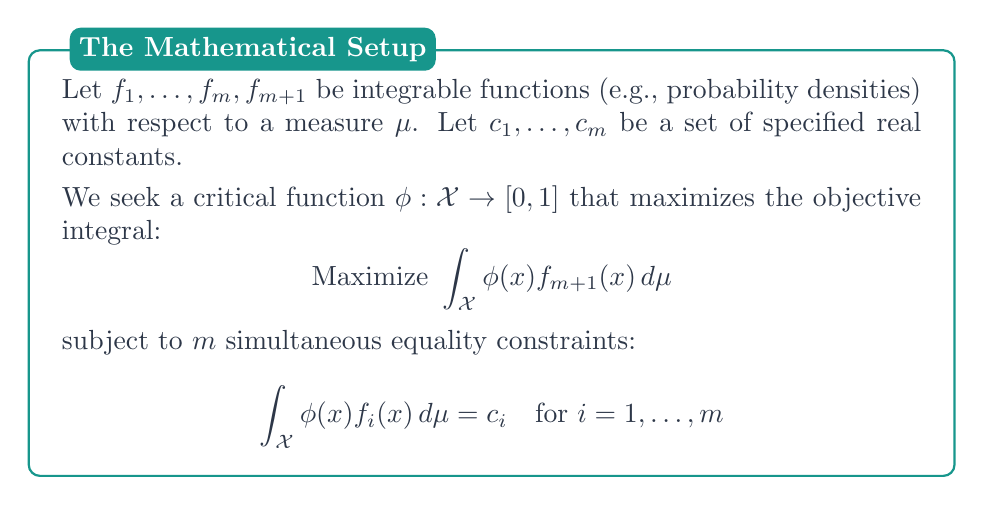
\begin{tikzpicture}
        % Reduced inner ysep to pull the bottom border up
        \node[draw=Teal, thick, rounded corners, inner xsep=12pt, inner ysep=10pt, fill=white] (box) {
            \begin{minipage}{0.9\textwidth}
                \color{Slate}
                Let $f_1, \dots, f_m, f_{m+1}$ be integrable functions (e.g., probability densities) with respect to a measure $\mu$. Let $c_1, \dots, c_m$ be a set of specified real constants.

                \smallskip % Swapped \vspace for a tighter \smallskip
                We seek a critical function $\phi: \mathcal{X} \to [0,1]$ that maximizes the objective integral:
                \[ \text{Maximize } \int_{\mathcal{X}} \phi(x) f_{m+1}(x) \, d\mu \]

                % Removed the extra \vspace here to tighten the layout
                subject to $m$ simultaneous equality constraints:
                \[ \int_{\mathcal{X}} \phi(x) f_i(x) \, d\mu = c_i \quad \text{for } i = 1, \dots, m \]
            \end{minipage}
        };
        % The colored banner on top of the border
        \node[fill=Teal, text=white, rounded corners, right=15pt] at (box.north west) {\bfseries The Mathematical Setup};
    \end{tikzpicture}
    \end{center}
\end{frame}

% --- Slide 9: Theorem 3.6.1 (Generalized Fundamental Lemma) 1/3 ---
\begin{frame}{Theorem 3.6.1 : Generalized Fundamental Lemma (1/3)}
    
    \lead{Theorem}\\
    \vspace{0.2cm}
    
    \noindent
    {\color{Teal}\vrule width 4pt}%
    \hspace{10pt}%
    \begin{minipage}{\dimexpr\textwidth-14pt\relax}
        \color{Slate}
        Let $(\mathcal{X}, \mathcal{F}, \mu)$ be a measure space. Let $f_1, f_2, \dots, f_m : \mathcal{X} \to \mathbb{R}$ be a set of constraint functions and let $f_{m+1} : \mathcal{X} \to \mathbb{R}$ be an objective function. All of these functions are integrable wrt $\mu$. Let $c_1, \dots, c_m \in \mathbb{R}$. Consider the class $\mathcal{C}$ defined as follows:
        \[
            \mathcal{C} \triangleq \left\{ \phi : \mathcal{X} \to [0,1] \;\middle|\; \int_{\mathcal{X}} \phi(x) f_i(x) \, d\mu(x) = c_i \quad \forall i \in \{1, \dots, m\} \right\}
        \]
        
        \vspace{0.1cm}
        Then:
        \vspace{0.2cm}
        \begin{itemize}
            \item[{\tikz[baseline=(char.base)]{\node[shape=circle,draw=Teal,inner sep=1pt,text=Teal,font=\scriptsize\bfseries] (char) {a};}}] \lead{Existence:} Among all valid tests in $\mathcal{C}$, there exists at least one optimal test that maximizes the objective integral $\displaystyle \int_{\mathcal{X}} \phi(x) f_{m+1}(x) \, d\mu(x)$.
        \end{itemize}
    \end{minipage}
\end{frame}

% --- Slide 10: Theorem 3.6.1 (Generalized Fundamental Lemma) 2/3 ---
\begin{frame}{Theorem 3.6.1 : Generalized Fundamental Lemma (2/3)}
    
    \noindent
    {\color{Teal}\vrule width 4pt}%
    \hspace{10pt}%
    \begin{minipage}{\dimexpr\textwidth-14pt\relax}
        \color{Slate}
        \begin{itemize}
            \item[{\tikz[baseline=(char.base)]{\node[shape=circle,draw=Teal,inner sep=1pt,text=Teal,font=\scriptsize\bfseries] (char) {b};}}] \lead{Sufficiency (The Blueprint):} A critical function $\phi \in \mathcal{C}$ is guaranteed to be this optimal maximizer if there exist constants $k_1, \dots, k_m \in \mathbb{R}$ such that
            \[
            \phi(x) = \begin{cases} 
            1, & \text{when } f_{m+1}(x) > \sum_{i=1}^m k_i f_i(x) \\[6pt]
            0, & \text{when } f_{m+1}(x) < \sum_{i=1}^m k_i f_i(x) 
            \end{cases}
            \]
            \textit{\{On the boundary, $\phi(x)$ can take any value between $[0,1]$.\}}
            
            \vspace{0.6cm}
            \item[{\tikz[baseline=(char.base)]{\node[shape=circle,draw=Teal,inner sep=1pt,text=Teal,font=\scriptsize\bfseries] (char) {c};}}] \lead{Inequality Constraints:} If the class $\mathcal{C}$ is instead defined by the inequality constraints $\displaystyle \int_{\mathcal{X}} \phi(x) f_i(x) \, d\mu(x) \le c_i \quad \forall i \in \{1 \dots m\}$, the exact same optimal structure from (b) applies, with the added restriction that the constants must be non-negative ($k_i \ge 0$).
        \end{itemize}
    \end{minipage}
\end{frame}

% --- Slide 11: Theorem 3.6.1 (Generalized Fundamental Lemma) 3/3 ---
\begin{frame}{Theorem 3.6.1 : Generalized Fundamental Lemma (3/3)}
    
    \noindent
    {\color{Teal}\vrule width 4pt}%
    \hspace{10pt}%
    \begin{minipage}{\dimexpr\textwidth-14pt\relax}
        \color{Slate}
        \begin{itemize}
            \item[{\tikz[baseline=(char.base)]{\node[shape=circle,draw=Teal,inner sep=1pt,text=Teal,font=\scriptsize\bfseries] (char) {d};}}] \lead{Necessity and Geometry:} Let $M$ be defined as the set of all possible constraint evaluations across \textbf{all} valid tests:
            \[ 
            M \triangleq \left\{ \left( \int_{\mathcal{X}} \phi f_1 \, d\mu, \dots, \int_{\mathcal{X}} \phi f_m \, d\mu \right) \;\middle|\; \phi : \mathcal{X} \to [0,1] \right\} 
            \]
            Then $M$ is closed and convex in $\mathbb{R}^m$. 
            
            \vspace{0.4cm}
            If $(c_1, \dots, c_m) \in \text{Int}(M)$, then the constants $k_1, \dots, k_m \in \mathbb{R}$ are guaranteed to exist and every optimal test $\phi$ must take the form described in (b) almost everywhere wrt $\mu$.
        \end{itemize}
    \end{minipage}
\end{frame}

% --- Slide 12: Proof Strategy ---
\begin{frame}{Proof Strategy for Theorem 3.6.1}
    \lead{Roadmap of the Proof}
    
    \vspace{0.4cm}
    We will decompose the proof of the Generalized Fundamental Lemma into four logical phases:
    
    \vspace{0.3cm}
    \begin{enumerate}
        \item \lead{Sufficiency (Part ii):} Direct algebraic verification showing that the structural form guarantees an optimal maximizer.
        \vspace{0.2cm}
        \item \lead{Inequality Constraints (Part iii):} Extending sufficiency to bounded constraint spaces.
        \vspace{0.2cm}
        \item \lead{Functional Analysis Preliminaries \& Existence (Part i):} Reviewing weak-$^\ast$ topology and compactness to guarantee an optimal test exists.
        \vspace{0.2cm}
        \item \lead{Necessity (Part iv):} Utilizing convex geometry and the Supporting Hyperplane Theorem to prove the optimal test must take this specific structural form.
    \end{enumerate}
\end{frame}

% --- Slide 13: Proof of Part (ii) - 1/4 (Setup) ---
\begin{frame}{Proof of Theorem 3.6.1: Part (ii) Sufficiency (1/4)}
    \lead{Objective:} Show that $\int \phi f_{m+1} \, d\mu \ge \int \phi^* f_{m+1} \, d\mu$ for any $\phi^* \in \mathcal{C}$.
    
    \vspace{0.5cm}
    Let $\phi^* \in \mathcal{C}$ be any other valid critical function. We construct a difference function to analyze their behavior across the space $\mathcal{X}$:
    \[ \Delta(x) \triangleq (\phi(x) - \phi^*(x)) \left[ f_{m+1}(x) - \sum_{i=1}^m k_i f_i(x) \right] \]
    
    \vspace{0.6cm}
    \lead{Claim:} The difference function $\Delta(x) \ge 0$ for all $x \in \mathcal{X}$.
\end{frame}

% --- Slide 14: Proof of Part (ii) - 2/4 (Diagram) ---
\begin{frame}{Proof of Theorem 3.6.1: Part (ii) Sufficiency (2/4)}
    To verify that $\Delta(x) \ge 0$ everywhere, we partition the sample space $\mathcal{X}$ into distinct regions based on the structural form of the optimal test $\phi(x)$.
    
    \vspace{0cm}
    % --- Image Placeholder ---
    % Replace the tikzpicture below with your actual image:
    % \includegraphics[width=0.7\textwidth, keepaspectratio]{your_ipad_diagram.png}
    \begin{center}
    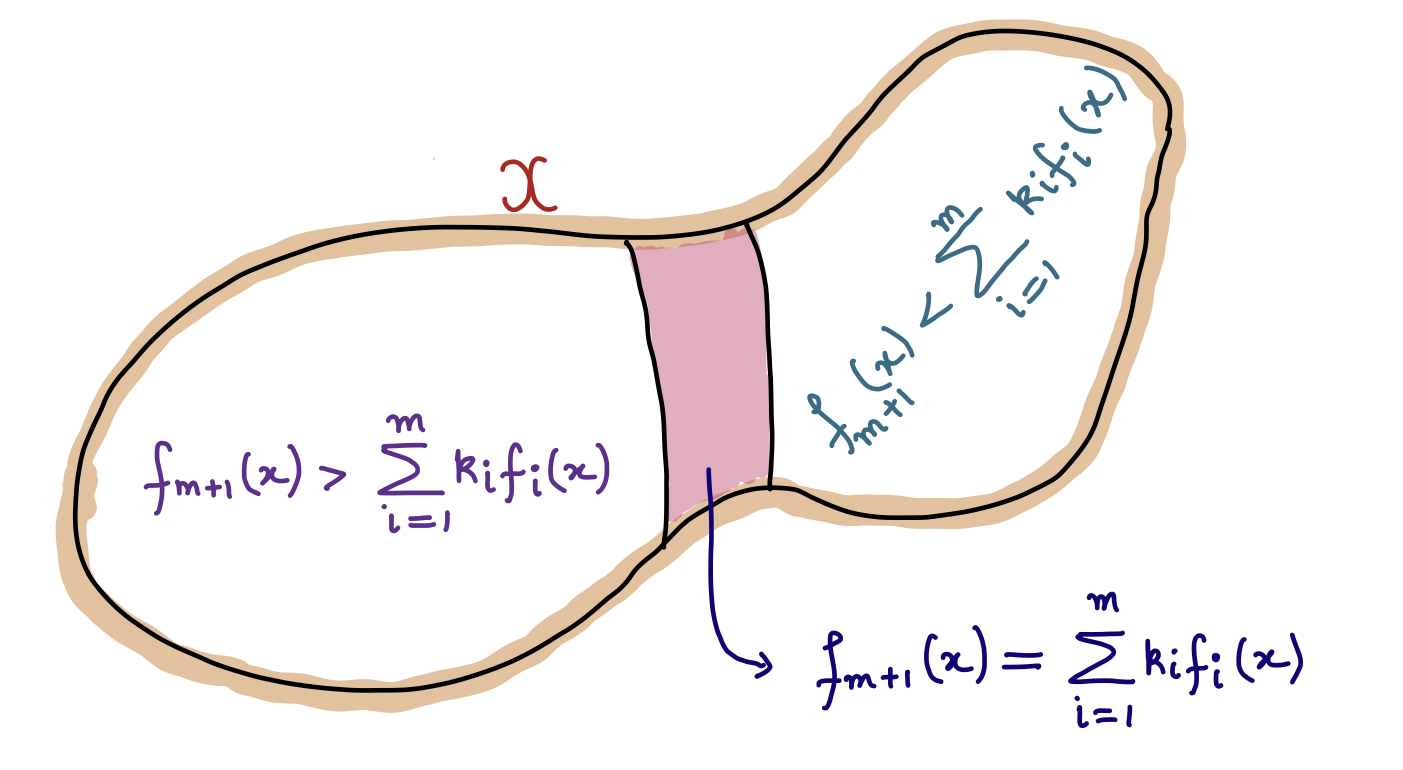
\includegraphics[width=0.75\textwidth, keepaspectratio]{partition.png}
    \end{center}
\end{frame}

% --- Slide 15: Proof of Part (ii) - 3/4 (Region Analysis) ---
\begin{frame}{Proof of Theorem 3.6.1: Part (ii) Sufficiency (3/4)}
    \begin{itemize}
        \item \lead{Region $R_1 \triangleq \{x \in \mathcal{X} : f_{m+1}(x) > \sum k_i f_i(x)\}$:}\\
        \vspace{0.1cm}
        Here, the optimal test dictates $\phi(x) = 1$. Since any valid test has $\phi^*(x) \in [0,1]$, we have $(\phi(x) - \phi^*(x)) \ge 0$. \\
        Thus, $\Delta(x) = (+\text{ve})(+\text{ve}) \ge 0$.
        
        \vspace{0.4cm}
        \item \lead{Region $R_2 \triangleq \{x \in \mathcal{X} : f_{m+1}(x) < \sum k_i f_i(x)\}$:}\\
        \vspace{0.1cm}
        Here, $\phi(x) = 0$. Since $\phi^*(x) \ge 0$, we have $(\phi(x) - \phi^*(x)) \le 0$. The second bracketed term is also strictly negative. \\
        Thus, $\Delta(x) = (-\text{ve})(-\text{ve}) \ge 0$.
        
        \vspace{0.4cm}
        \item \lead{Boundary Region:}\\
        \vspace{0.1cm}
        Where $f_{m+1}(x) = \sum k_i f_i(x)$, the second bracketed term is exactly $0$, forcing $\Delta(x) = 0$.
    \end{itemize}
\end{frame}

% --- Slide 16: Proof of Part (ii) - 4/4 (Integration & Conclusion) ---
\begin{frame}{Proof of Theorem 3.6.1: Part (ii) Sufficiency (4/4)}
    Since $\Delta(x) \ge 0$ everywhere, its Lebesgue integral must be non-negative:
    \[ \int_{\mathcal{X}} \Delta(x) \, d\mu(x) \ge 0 \]
    
    \vspace{0.2cm}
    Expanding the integral by linearity and distributing over the test functions yields:
    \[ \int_{\mathcal{X}} (\phi - \phi^*) f_{m+1} \, d\mu - \sum_{i=1}^m k_i \left( \int_{\mathcal{X}} \phi f_i \, d\mu - \int_{\mathcal{X}} \phi^* f_i \, d\mu \right) \ge 0 \]
    
    \vspace{0.3cm}
    Because both $\phi, \phi^* \in \mathcal{C}$, they satisfy the exact same constraints ($c_i$). The difference inside the summation is exactly $(c_i - c_i = 0)$. 
    
    \vspace{0.3cm}
    The summation term vanishes entirely, leaving:
    \[ \int_{\mathcal{X}} (\phi - \phi^*) f_{m+1} \, d\mu \ge 0 \implies \int_{\mathcal{X}} \phi f_{m+1} \, d\mu \ge \int_{\mathcal{X}} \phi^* f_{m+1} \, d\mu \qed \]
\end{frame}

% --- Slide 17: Proof of Part (iii) - 1/4 (Setup & Constraint Space) ---
\begin{frame}{Proof of Theorem 3.6.1: Part (iii) Inequality Constraints (1/4)}
    \lead{Objective:} Prove that the optimal structure still holds if the class $\mathcal{C}$ is defined by inequality constraints, provided the constants are non-negative.
    
    \vspace{0.5cm}
    \begin{center}
    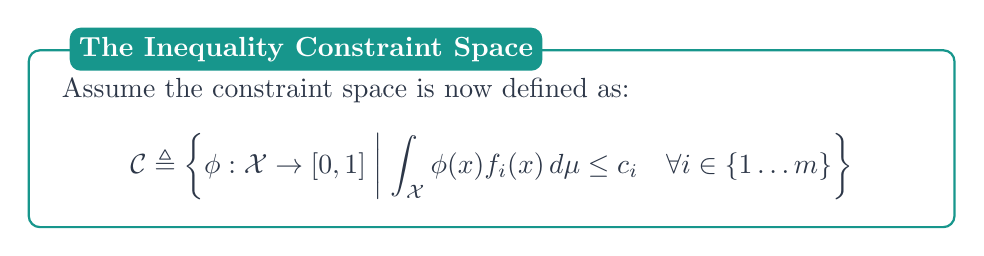
\begin{tikzpicture}
        \node[draw=Teal, thick, rounded corners, inner xsep=12pt, inner ysep=10pt, fill=white] (box) {
            \begin{minipage}{0.9\textwidth}
                \color{Slate}
                Assume the constraint space is now defined as:
                \[ \mathcal{C} \triangleq \left\{ \phi : \mathcal{X} \to [0,1] \;\middle|\; \int_{\mathcal{X}} \phi(x) f_i(x) \, d\mu \le c_i \quad \forall i \in \{1 \dots m\} \right\} \]
            \end{minipage}
        };
        \node[fill=Teal, text=white, rounded corners, right=15pt] at (box.north west) {\bfseries The Inequality Constraint Space};
    \end{tikzpicture}
    \end{center}
\end{frame}

% --- Slide 18: Proof of Part (iii) - 2/4 (The Test Functions) ---
\begin{frame}{Proof of Theorem 3.6.1: Part (iii) Inequality Constraints (2/4)}
    Let $\phi \in \mathcal{C}$ be a specific test function that satisfies the constraints \textbf{exactly}:
    \[ \int_{\mathcal{X}} \phi(x) f_i(x) \, d\mu = c_i \quad \forall i \in \{1 \dots m\} \]
    and assume there exist non-negative constants $k_1, \dots, k_m \ge 0$ such that $\phi$ takes the standard optimal structural form.
    
    \vspace{0.6cm}
    Let $\phi^* \in \mathcal{C}$ be any other competing test function in this inequality-bounded space. By definition, this means:
    \[ \int_{\mathcal{X}} \phi^*(x) f_i(x) \, d\mu \le c_i \quad \forall i \in \{1 \dots m\} \]
\end{frame}

% --- Slide 19: Proof of Part (iii) - 3/4 (Algebraic Substitution) ---
\begin{frame}{Proof of Theorem 3.6.1: Part (iii) Inequality Constraints (3/4)}
    From the proof of Part (ii), the non-negativity of the difference function $\Delta(x)$ led us to the following fundamental inequality \textit{before} we assumed $c_i - c_i = 0$:
    
    \vspace{0.1cm}
    \[ 
        \int_{\mathcal{X}} (\phi - \phi^*) f_{m+1} \, d\mu \ge \sum_{i=1}^m k_i \left( \int_{\mathcal{X}} \phi f_i \, d\mu - \int_{\mathcal{X}} \phi^* f_i \, d\mu \right)
    \]
    
    \vspace{0.3cm}
    We substitute the exact equality $\int \phi f_i \, d\mu = c_i$ into the right-hand side of our inequality:
    
    \vspace{0.1cm}
    \[
        \int_{\mathcal{X}} (\phi - \phi^*) f_{m+1} \, d\mu \ge \sum_{i=1}^m \underbrace{k_i}_{\ge \, 0} \Biggl( \underbrace{ c_i - \underbrace{\int_{\mathcal{X}} \phi^* f_i \, d\mu}_{\le \, c_i} }_{\ge \, 0} \Biggr)
    \]
\end{frame}

% --- Slide 20: Proof of Part (iii) - 4/4 (Sign Analysis & Conclusion) ---
\begin{frame}{Proof of Theorem 3.6.1: Part (iii) Inequality Constraints (4/4)}
    \lead{Sign Analysis:}\\
    \vspace{0.2cm}
    \begin{itemize}
        \item We are explicitly given that the constants are non-negative ($k_i \ge 0$).
        \vspace{0.3cm}
        \item Because $\phi^* \in \mathcal{C}$, we know its integral is bounded by $c_i$, making the difference $(c_i - \int \phi^* f_i) \ge 0$.
    \end{itemize}
    
    \vspace{0.6cm}
    Since every term in the sum is the product of two non-negative numbers, the entire summation is strictly $\ge 0$. Thus:
    
    \vspace{0.2cm}
    \[
        \int_{\mathcal{X}} (\phi - \phi^*) f_{m+1} \, d\mu \ge 0 \implies \int_{\mathcal{X}} \phi f_{m+1} \, d\mu \ge \int_{\mathcal{X}} \phi^* f_{m+1} \, d\mu \qed
    \]
\end{frame}

% --- Slide 21: Functional Analysis Preliminaries: L-Spaces ---
\begin{frame}{Functional Analysis Preliminaries (1/2)}
    \lead{The $L_1$ and $L_\infty$ Banach Spaces}\\
    Let $(\mathcal{X}, \mathcal{F}, \mu)$ be a $\sigma$-finite measure space. We define these spaces formally as equivalence classes of functions (where $f \equiv g$ if $f = g$ $\mu$-a.e.):
    
    \vspace{0.2cm}
    \begin{itemize}
        \item[{ \tikz\fill[Teal] (0,0) circle (2pt); }] \lead{The Space $L_1(\mathcal{X}, \mu)$:} The space of absolutely integrable functions, bounded by the $L_1$-norm:
        \[ L_1(\mathcal{X}, \mu) \triangleq \left\{ f : \mathcal{X} \to \mathbb{R} \;\middle|\; \|f\|_1 = \int_{\mathcal{X}} |f(x)| \, d\mu < \infty \right\} \]
        
        \vspace{0.1cm}
        \item[{ \tikz\fill[Teal] (0,0) circle (2pt); }] \lead{The Space $L_\infty(\mathcal{X}, \mu)$:} The space of essentially bounded functions, bounded by the $L_\infty$-norm:
        \[ L_\infty(\mathcal{X}, \mu) \triangleq \left\{ \phi : \mathcal{X} \to \mathbb{R} \;\middle|\; \|\phi\|_\infty = \operatorname*{ess\,sup}_{x \in \mathcal{X}} |\phi(x)| < \infty \right\} \]
    \end{itemize}

    \vspace{0.2cm}
    \lead{Duality:}\\
    $L_\infty(\mathcal{X}, \mu)$ is the continuous dual space of $L_1(\mathcal{X}, \mu)$.
\end{frame}
% --- Slide 22: Functional Analysis Preliminaries: Weak-* & Banach-Alaoglu ---
\begin{frame}{Functional Analysis Preliminaries (2/2)}
\lead{Weak-$^\ast$ Convergence}\\
    \vspace{0.1cm}
    \noindent
    {\color{Teal}\vrule width 4pt}%
    \hspace{10pt}%
    \begin{minipage}{\dimexpr\textwidth-14pt\relax}
        \color{Slate}
        A sequence $\{\phi_n\} \subset L_\infty(\mathcal{X}, \mu)$ converges weak-$^\ast$ to $\phi \in L_\infty(\mathcal{X}, \mu)$ if and only if:
        \[ \lim_{n \to \infty} \int_{\mathcal{X}} \phi_n(x) f(x) \, d\mu = \int_{\mathcal{X}} \phi(x) f(x) \, d\mu \quad \forall f \in L_1(\mathcal{X}, \mu) \]
        
        \vspace{0.1cm}
        \textit{Insight:} This implies that integration with an $L_1$ function acts as a continuous operation in the weak-$^\ast$ topology.
    \end{minipage}
    
    \vspace{0.6cm}
    \lead{Theorem (Banach-Alaoglu)}\\
    \vspace{0.1cm}
    \noindent
    {\color{Teal}\vrule width 4pt}%
    \hspace{10pt}%
    \begin{minipage}{\dimexpr\textwidth-14pt\relax}
        \color{Slate}
        Let $X$ be a normed vector space and let $X^*$ be its continuous dual space. 
        
        \vspace{0.1cm}
        The closed unit ball in the dual space, defined as:
        \[ B_{X^*} \triangleq \{ \phi \in X^* : \|\phi\|_{X^*} \le 1 \} \]
        is \textbf{compact} with respect to the weak-$^\ast$ topology. 
    \end{minipage}
\end{frame}

% --- Slide 24: Proof of Part (i) - 1/5 (Objective & Strategy) ---
\begin{frame}{Proof of Theorem 3.6.1: Part (i) Existence (1/5)}
    \lead{Objective:} Prove that among all valid tests satisfying the constraints $\int \phi f_i d\mu = c_i$, there exists at least one optimal test that maximizes the objective integral $\int \phi f_{m+1} d\mu$.
    
    \vspace{0.2cm}
    \lead{Proof Strategy:}\\
    \vspace{0.1cm}
    We will prove existence by translating the problem into functional analysis and relying on topological compactness:
    
    \vspace{0.1cm}
    \begin{itemize}
        \item[{ \tikz\fill[Teal] (0,0) circle (2pt); }] \textbf{Step 1:} Show the space of all valid tests $\Phi$ is compact in the weak-$^\ast$ topology using the Banach-Alaoglu Theorem.
        \vspace{0.1cm}
        \item[{ \tikz\fill[Teal] (0,0) circle (2pt); }] \textbf{Step 2:} Define integration as a continuous mapping to prove the restricted constraint space $\mathcal{C}_{a.e.}$ is a closed subset, and thus compact.
        \vspace{0.1cm}
        \item[{ \tikz\fill[Teal] (0,0) circle (2pt); }] \textbf{Step 3:} Apply the Extreme Value Theorem to the objective integral to guarantee a maximizer exists in $\mathcal{C}_{a.e.}$.
        \vspace{0.1cm}
        \item[{ \tikz\fill[Teal] (0,0) circle (2pt); }] \textbf{Step 4:} Fix the boundary behavior (measure zero sets) to ensure the test is strictly bounded in $[0,1]$ everywhere.
    \end{itemize}
\end{frame}

% --- Slide 25: Proof of Part (i) - 2/5 (Compactness of Phi) ---
\begin{frame}{Proof of Theorem 3.6.1: Part (i) Existence (2/5)}
    \lead{Step 1: Compactness of the Test Space $\Phi$}\\
    \vspace{0.2cm}
    Let $B \triangleq \{ \phi \in L^\infty(\mathcal{X}, \mu) \mid \|\phi\|_\infty \le 1 \}$ be the closed unit ball. By the Banach-Alaoglu theorem, $B$ is compact in the weak-$^\ast$ topology.
    
    \vspace{0.4cm}
    Define the set of all valid test functions (up to almost everywhere equivalence):
    \[ \Phi = \{ \phi : \mathcal{X} \to \mathbb{R} \mid 0 \le \phi(x) \le 1 \text{ a.e.} \} \]
    
    \vspace{0.3cm}
    \noindent
    {\color{Teal}\vrule width 4pt}%
    \hspace{10pt}%
    \begin{minipage}{\dimexpr\textwidth-14pt\relax}
        \color{Slate}
        We can express $\Phi$ as the intersection of the unit ball $B$ with the set of non-negative functions:
        \[ \Phi = B \cap \{ \phi \in L^\infty(\mathcal{X}, \mu) \mid \phi(x) \ge 0 \text{ a.e.} \} \]
        Because $\Phi$ is a closed subset of the compact set $B$, $\Phi$ itself must be weakly-$^\ast$ compact.
    \end{minipage}
\end{frame}

% --- Slide 26: Proof of Part (i) - 3/5 (Constraint Space) ---
\begin{frame}{Proof of Theorem 3.6.1: Part (i) Existence (3/5)}
    \lead{Step 2: Compactness of the Constraint Space}
    
    \vspace{0.1cm}
    Consider the mapping $N_f : L^\infty(\mathcal{X}, \mu) \to \mathbb{R}$ defined by the integral:
    \[ N_f(\phi) \triangleq \int_{\mathcal{X}} \phi f \, d\mu \]
    Since $f \in L_1$, $N_f$ is a continuous map under the weak-$^\ast$ topology.
    
    \vspace{0.2cm}
    For each constraint $i \in \{1 \dots m\}$, the singleton set $\{c_i\} \subset \mathbb{R}$ is closed. Therefore, its pre-image $N_{f_i}^{-1}(\{c_i\})$ is a closed set.
    
    \vspace{0.2cm}
    We define our specific constraint class almost everywhere as:
    \[ \mathcal{C}_{a.e.} = \left\{ \phi \in \Phi \;\middle|\; \int_{\mathcal{X}} \phi f_i \, d\mu = c_i \quad \forall i \in \{1 \dots m\} \right\} = \Phi \cap \left( \bigcap_{i=1}^m N_{f_i}^{-1}(\{c_i\}) \right) \]
    
    \vspace{0.1cm}
    Being an intersection of closed sets with the compact set $\Phi$, $\mathcal{C}_{a.e.}$ is \textbf{compact}.
\end{frame}

% --- Slide 27: Proof of Part (i) - 4/5 (Extreme Value Theorem) ---
\begin{frame}{Proof of Theorem 3.6.1: Part (i) Existence (4/5)}
    \lead{Step 3: Applying the Extreme Value Theorem}
    
    \vspace{0.3cm}
    Now consider our primary objective functional $N_{f_{m+1}} : L^\infty(\mathcal{X}, \mu) \to \mathbb{R}$ defined as:
    \[ N_{f_{m+1}}(\phi) \triangleq \int_{\mathcal{X}} \phi f_{m+1} \, d\mu \]
    
    \vspace{0.3cm}
    \begin{itemize}
        \item[{ \tikz\fill[Teal] (0,0) circle (2pt); }] Because $f_{m+1} \in L_1(\mathcal{X}, \mu)$, the map $N_{f_{m+1}}$ is weak-$^\ast$ continuous.
        \vspace{0.2cm}
        \item[{ \tikz\fill[Teal] (0,0) circle (2pt); }] The domain $\mathcal{C}_{a.e.}$ over which we are maximizing is weak-$^\ast$ compact.
    \end{itemize}
    
    \vspace{0.4cm}
    \noindent
    {\color{Teal}\vrule width 4pt}%
    \hspace{10pt}%
    \begin{minipage}{\dimexpr\textwidth-14pt\relax}
        \color{Slate}
        \textbf{Extreme Value Theorem:}\\
        A continuous real-valued function on a compact space attains its maximum. Therefore, there must exist a function $\phi^* \in \mathcal{C}_{a.e.}$ that maximizes $N_{f_{m+1}}(\phi^*)$.
    \end{minipage}
\end{frame}

% --- Slide 28: Proof of Part (i) - 5/5 (Fixing Measure Zero) ---
\begin{frame}{Proof of Theorem 3.6.1: Part (i) Existence (5/5)}
    \lead{Step 4: Fixing the Measure Zero Boundary}
    
    \vspace{0.2cm}
    The maximizer $\phi^*$ is bounded between $[0,1]$ \textit{almost everywhere}. To make it a strictly valid test \textit{everywhere}, we define $\tilde{\phi}^* : \mathcal{X} \to [0,1]$ as:
    \[
    \tilde{\phi}^*(x) = \begin{cases} 
    \phi^*(x), & \text{if } \phi^*(x) \in [0,1] \\
    1, & \text{if } \phi^*(x) > 1 \\
    0, & \text{if } \phi^*(x) < 0 
    \end{cases}
    \]
    
    \vspace{0.1cm}
    Because $\phi^* \in \Phi$, the set of points where $\phi^*(x) > 1$ or $\phi^*(x) < 0$ has measure zero. Thus, $\phi^*$ and $\tilde{\phi}^*$ are equal almost everywhere. This guarantees the exact integrals are preserved:
    \[ \int_{\mathcal{X}} \tilde{\phi}^* f_i \, d\mu = \int_{\mathcal{X}} \phi^* f_i \, d\mu = c_i \quad \text{(Constraints met)} \]
    \[ \int_{\mathcal{X}} \tilde{\phi}^* f_{m+1} \, d\mu = \int_{\mathcal{X}} \phi^* f_{m+1} \, d\mu \quad \text{(Objective maximized)} \]
    Thus, the strictly valid optimal test $\tilde{\phi}^*$ exists. \qed
\end{frame}

% --- Slide 29: Towards Part (iv) - Convex Sets ---
\begin{frame}{Towards part (iv): Convex Geometry (1/3)}
    \lead{Convex Sets in $\mathbb{R}^m$}\\
    \vspace{0.2cm}
    \noindent
    {\color{Teal}\vrule width 4pt}%
    \hspace{10pt}%
    \begin{minipage}{\dimexpr\textwidth-14pt\relax}
        \color{Slate}
        \textbf{Definition (Convex Set):}\\
        \vspace{0.1cm}
        A set $M \subset \mathbb{R}^m$ is called \textbf{convex} if, for any two points $u, v \in M$ and any scalar $\alpha \in [0,1]$, the line segment connecting them is also entirely contained within $M$:
        \[ \alpha u + (1-\alpha) v \in M \]
    \end{minipage}

    \vspace{0.6cm}
    \lead{Interior and Boundary}\\
    \vspace{0.2cm}
    \begin{itemize}
        \item[{ \tikz\fill[Teal] (0,0) circle (2pt); }] The interior of $M$, denoted $\text{Int}(M)$, is the set of all points in $M$ that possess an open neighborhood completely contained within $M$.
        \vspace{0.2cm}
        \item[{ \tikz\fill[Teal] (0,0) circle (2pt); }] A point $y \in \mathbb{R}^m$ lies on the boundary of $M$ if every neighborhood of $y$ contains both points in $M$ and points outside of $M$.
    \end{itemize}
\end{frame}

% --- Slide 30: Towards Part (iv) - Supporting Hyperplane ---
\begin{frame}{Towards part (iv): Supporting Hyperplane Theorem (2/3)}
    \lead{Theorem (Supporting Hyperplane)}\\
    \vspace{0.4cm}
    \noindent
    {\color{Teal}\vrule width 4pt}%
    \hspace{10pt}%
    \begin{minipage}{\dimexpr\textwidth-14pt\relax}
        \color{Slate}
        Let $M \subset \mathbb{R}^m$ be a convex set, and let $y \in \mathbb{R}^m$ be a point that does not belong to the interior of $M$ (i.e., $y \notin \text{Int}(M)$). 
        
        \vspace{0.4cm}
        Then, there exists a non-zero vector $a \in \mathbb{R}^m \setminus \{0\}$ such that the hyperplane defined by the normal vector $a$ bounds the set $M$:
        \[ \langle a, x \rangle \le \langle a, y \rangle \quad \forall x \in M \]
        
        \vspace{0.2cm}
        Equivalently, expressing the Euclidean inner product as a sum:
        \[ \sum_{i=1}^m a_i x_i \le \sum_{i=1}^m a_i y_i \quad \forall x \in M \]
    \end{minipage}
\end{frame}

% --- Slide 31: Towards Part (iv) - Geometric Intuition ---
\begin{frame}{Towards part (iv): Supporting Hyperplane Theorem (3/3)}
    \lead{Geometric Intuition}\\
    \vspace{0.2cm}
    The vector $a$ acts as the normal to a hyperplane passing through $y$. The entire convex set $M$ lies in the negative half-space generated by this hyperplane.
    
    \vspace{0.4cm}
    \begin{center}
        % Constraining by height instead of width for portrait-oriented images
        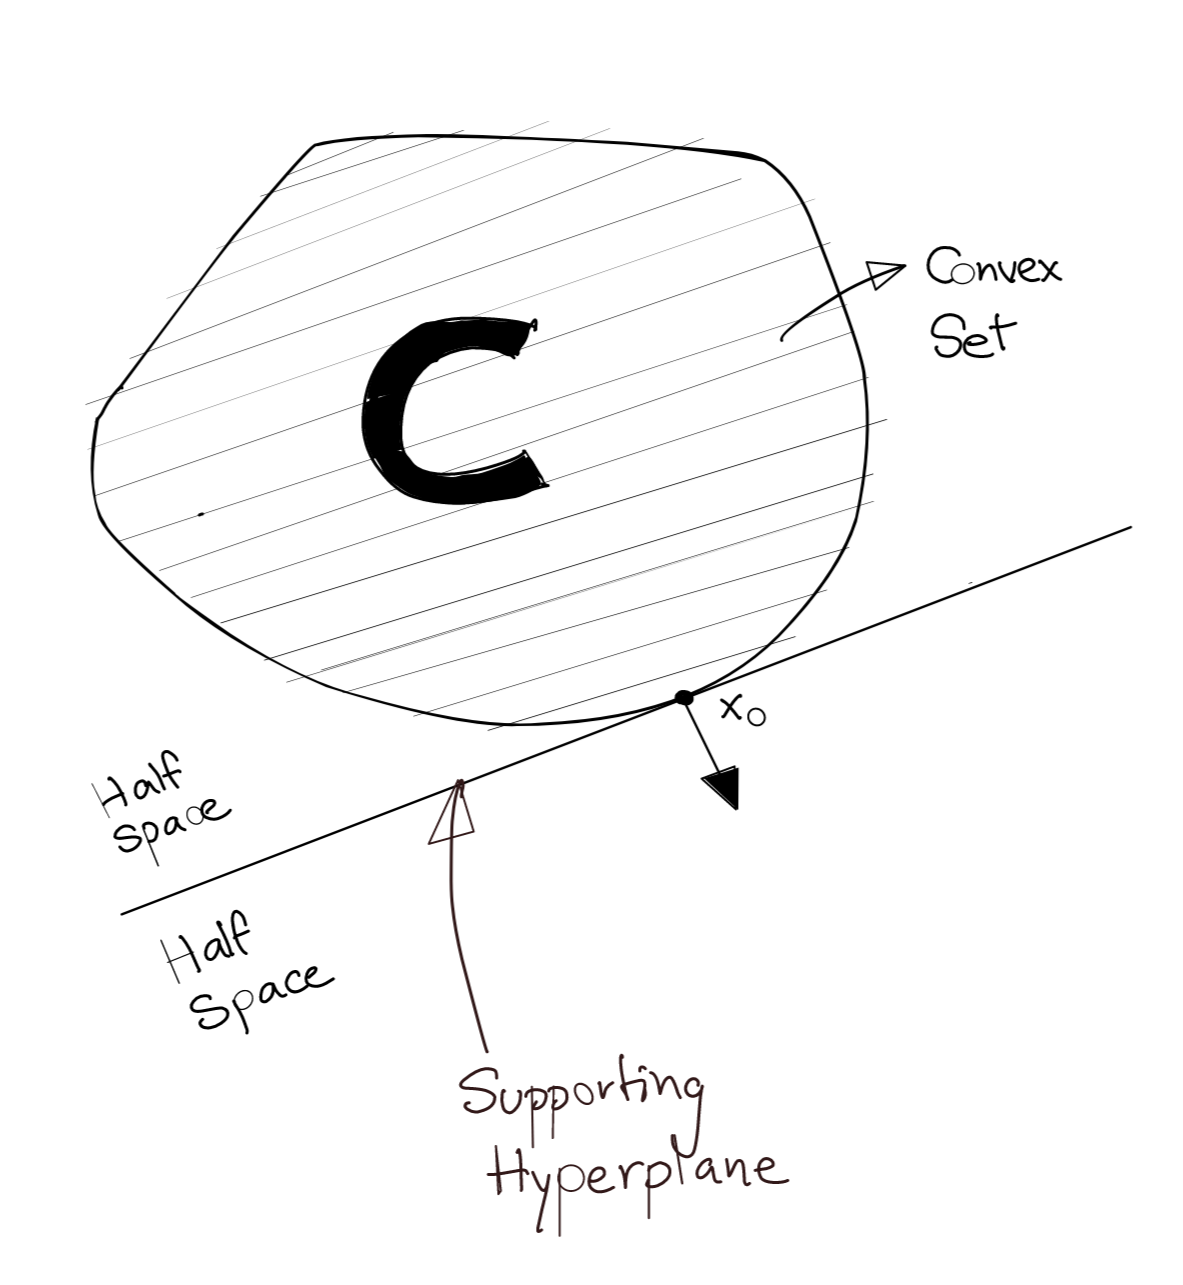
\includegraphics[height=0.55\textheight, keepaspectratio]{hyperplane.png}
    \end{center}
\end{frame}

% --- Slide 32: Proof of Part (iv) - Strategy 1/4 ---
\begin{frame}{Proof of Theorem 3.6.1: Part (iv) Necessity (Strategy 1/4)}
    \lead{Objective:} Prove that if an optimal test $\phi^*$ exists and the constraint vector $c \in \text{Int}(M)$, then $\phi^*$ \textit{must} take the standard structural form $\mu$-a.e.

    \vspace{0.4cm}
    \lead{Attacking Plan:}\\
    \vspace{0.2cm}
    \begin{itemize}
        \item[{ \tikz\fill[Teal] (0,0) circle (2pt); }] \textbf{Step 1: Mapping to Euclidean Space}\\
        Define image sets for the tests under our integral mappings:
        \[ M \triangleq \left\{ \left( \int_{\mathcal{X}} \phi f_1 \, d\mu, \dots, \int_{\mathcal{X}} \phi f_m \, d\mu \right) \;\middle|\; \phi \in \Phi \right\} \subset \mathbb{R}^m \]
        and similarly define $S \subset \mathbb{R}^{m+1}$ by including the objective integral $\int \phi f_{m+1} d\mu$. We will first prove $M$ and $S$ are compact and convex.
    \end{itemize}
\end{frame}

% --- Slide 33: Proof of Part (iv) - Strategy 2/4 ---
\begin{frame}{Proof of Theorem 3.6.1: Part (iv) Necessity (Strategy 2/4)}
    \lead{Attacking Plan (Continued):}\\
    \vspace{0.4cm}
    \begin{itemize}
        \item[{ \tikz\fill[Teal] (0,0) circle (2pt); }] \textbf{Step 2: Supporting Hyperplane}\\
        Show the optimal test maps to a boundary point $p^* \in \partial S$. Apply the Supporting Hyperplane Theorem to find a separating normal vector $w$:
        \[ \exists w \in \mathbb{R}^{m+1} \setminus \{0\} \text{ s.t. } \langle w, s \rangle \le \langle w, p^* \rangle \quad \forall s \in S \]
        
        \vspace{0.6cm}
        \item[{ \tikz\fill[Teal] (0,0) circle (2pt); }] \textbf{Step 3: Objective Weight Positivity}\\
        Exploit the interior hypothesis $c \in \text{Int}(M)$ to strictly prove that the weight corresponding to the objective function is strictly positive:
        \[ w_{m+1} > 0 \]
    \end{itemize}
\end{frame}

% --- Slide 34: Proof of Part (iv) - Strategy 3/4 ---
\begin{frame}{Proof of Theorem 3.6.1: Part (iv) Necessity (Strategy 3/4)}
    \lead{Attacking Plan (Continued):}\\
    \vspace{0.4cm}
    \begin{itemize}
        \item[{ \tikz\fill[Teal] (0,0) circle (2pt); }] \textbf{Step 4: Algebraic Reduction}\\
        Since $w_{m+1} > 0$, divide the fundamental inequality $\langle w, s \rangle \le \langle w, p^* \rangle$ by $w_{m+1}$. 
        
        \vspace{0.4cm}
        Define the constants $k_i \triangleq -w_i / w_{m+1}$ for $i \in \{1 \dots m\}$. By substituting the integrals back in, reduce the summation to a single bounded integral over $\mathcal{X}$:
        \[ \int_{\mathcal{X}} (\phi - \phi^*) \underbrace{\left( f_{m+1} - \sum_{i=1}^m k_i f_i \right)}_{\triangleq \, g(x)} d\mu \le 0 \quad \forall \phi \in \Phi \]
    \end{itemize}
\end{frame}

% --- Slide 35: Proof of Part (iv) - Strategy 4/4 ---
\begin{frame}{Proof of Theorem 3.6.1: Part (iv) Necessity (Strategy 4/4)}
    \lead{Attacking Plan (Continued):}\\
    \vspace{0.4cm}
    \begin{itemize}
        \item[{ \tikz\fill[Teal] (0,0) circle (2pt); }] \textbf{Step 5: Measure-Theoretic Necessity}\\
        Analyze the sign of the inner function $g(x)$. Use contradiction on arbitrary subsets $A \subset \mathcal{X}$ with strictly positive measure ($\mu(A) > 0$) to force the required structure:
        \[ \phi^*(x) = \begin{cases} 1, & \text{if } g(x) > 0 \\ 0, & \text{if } g(x) < 0 \end{cases} \quad \mu\text{-a.e.} \]
        
        \vspace{0.2cm}
        This guarantees the optimal test must match the generalized Neyman-Pearson structural form almost everywhere.
    \end{itemize}
\end{frame}

% --- Slide 36: Proof of Part (iv) - Step 1 (Definitions) ---
\begin{frame}{Proof of Theorem 3.6.1: Part (iv) Necessity (Step 1 - 1/4)}
    \lead{Step 1: The Geometry of Integrals - Defining the Image Sets}\\
    \vspace{0.2cm}
    We map the infinite-dimensional test space $\Phi$ into finite-dimensional Euclidean spaces by evaluating the constraint and objective integrals.
    
    \vspace{0.4cm}
    \begin{itemize}
        \item[{ \tikz\fill[Teal] (0,0) circle (2pt); }] \textbf{The Constraint Set $M$:}
        \[ M \triangleq \left\{ \left( \int_{\mathcal{X}} \phi f_1 \, d\mu, \dots, \int_{\mathcal{X}} \phi f_m \, d\mu \right) \;\middle|\; \phi \in \Phi \right\} \subset \mathbb{R}^m \]
        
        \vspace{0.4cm}
        \item[{ \tikz\fill[Teal] (0,0) circle (2pt); }] \textbf{The Extended Set $S$:}
        \[ S \triangleq \left\{ \left( \int_{\mathcal{X}} \phi f_1 \, d\mu, \dots, \int_{\mathcal{X}} \phi f_{m+1} \, d\mu \right) \;\middle|\; \phi \in \Phi \right\} \subset \mathbb{R}^{m+1} \]
    \end{itemize}
\end{frame}

% --- Slide 37: Proof of Part (iv) - Step 1 (Convexity) ---
\begin{frame}{Proof of Theorem 3.6.1: Part (iv) Necessity (Step 1 - 2/4)}
    \lead{Step 1: Convexity of $M$ and $S$}\\
    \vspace{0.4cm}
    
    First, observe that the space of all valid tests $\Phi$ is a \textbf{convex set}. For any $\phi_1, \phi_2 \in \Phi$ and scalar $\alpha \in [0,1]$:
    \[ 0 \le \alpha \phi_1(x) + (1-\alpha)\phi_2(x) \le 1 \quad \mu\text{-a.e.} \]
    
    \vspace{0.4cm}
    Next, consider the mapping $\phi \mapsto \int_{\mathcal{X}} \phi f_i \, d\mu$. Because the Lebesgue integral is a strictly \textbf{linear operator}, the sets $M$ and $S$ are generated by applying a linear transformation to a convex set.
    
    \vspace{0.4cm}
    \noindent
    {\color{Teal}\vrule width 4pt}%
    \hspace{10pt}%
    \begin{minipage}{\dimexpr\textwidth-14pt\relax}
        \color{Slate}
        \textbf{Conclusion 1:}\\
        The image of a convex set under a linear map is always convex. Thus, both $M$ and $S$ are \textbf{convex sets} in $\mathbb{R}^m$ and $\mathbb{R}^{m+1}$.
    \end{minipage}
\end{frame}

% --- Slide 38: Proof of Part (iv) - Step 1 (Continuity & Compactness) ---
\begin{frame}{Proof of Theorem 3.6.1: Part (iv) Necessity (Step 1 - 3/4)}
    \lead{Step 1: Topological Compactness of $M$ and $S$}\\
    \vspace{0.4cm}
    
    Recall from our functional analysis prerequisites:
    \vspace{0.2cm}
    \begin{enumerate}
        \item The test space $\Phi$ is \textbf{compact} in the weak-$^\ast$ topology (Banach-Alaoglu).
        \vspace{0.3cm}
        \item Because each $f_i \in L_1(\mathcal{X}, \mu)$, the mapping $\phi \mapsto \int_{\mathcal{X}} \phi f_i \, d\mu$ is \textbf{continuous} with respect to the weak-$^\ast$ topology.
    \end{enumerate}
    
    \vspace{0.5cm}
    Because the individual component functions are continuous, the vector-valued coordinate mappings $\Phi \to \mathbb{R}^m$ and $\Phi \to \mathbb{R}^{m+1}$ that construct $M$ and $S$ are continuous.
\end{frame}

% --- Slide 39: Proof of Part (iv) - Step 1 (Heine-Borel) ---
\begin{frame}{Proof of Theorem 3.6.1: Part (iv) Necessity (Step 1 - 4/4)}
    \lead{Step 1: Applying the Heine-Borel Theorem}\\
    \vspace{0.4cm}
    
    A fundamental topological theorem states that the continuous image of a compact space is necessarily compact. 
    
    \vspace{0.2cm}
    Since $\Phi$ is compact, its images $M$ and $S$ must also be \textbf{compact sets} within their respective Euclidean spaces.
    
    \vspace{0.4cm}
    \noindent
    {\color{Teal}\vrule width 4pt}%
    \hspace{10pt}%
    \begin{minipage}{\dimexpr\textwidth-14pt\relax}
        \color{Slate}
        \textbf{Theorem (Heine-Borel):}\\
        In finite-dimensional Euclidean space, a set is compact if and only if it is both \textbf{closed} and \textbf{bounded}.
        
        \vspace{0.3cm}
        \textbf{Final Conclusion of Step 1:}\\
        The sets $M$ and $S$ are strictly closed, bounded, and convex. (This geometrical structure is required to invoke the Supporting Hyperplane Theorem in Step 2).
    \end{minipage}
\end{frame}

% --- Slide 40: Proof of Part (iv) - Step 2 (Defining the Optimal Point) ---
\begin{frame}{Proof of Theorem 3.6.1: Part (iv) Necessity (Step 2 - 1/5)}
    \lead{Step 2: Constructing the Optimal Point in $S$}\\
    \vspace{0.4cm}
    
    By our primary hypothesis, the constraint vector $c = (c_1, \dots, c_m)$ is strictly an interior point of the constraint space $M$.
    
    \vspace{0.4cm}
    Let $\phi^* \in \Phi$ be the specific test function that \textit{maximizes} the objective integral while satisfying these constraints. We define this maximum objective value as $c^*_{m+1}$:
    \[ c^*_{m+1} \triangleq \int_{\mathcal{X}} \phi^* f_{m+1} \, d\mu \]
    
    We can now map this optimal test $\phi^*$ into our extended Euclidean set $S \subset \mathbb{R}^{m+1}$. Let $p^*$ be the image of $\phi^*$:
    \[ p^* \triangleq \left( \int_{\mathcal{X}} \phi^* f_1 \, d\mu, \dots, \int_{\mathcal{X}} \phi^* f_{m+1} \, d\mu \right) = (c_1, c_2, \dots, c_m, c^*_{m+1}) \]
    Since $\phi^* \in \Phi$, it immediately follows that $p^* \in S$.
\end{frame}

% --- Slide 41: Proof of Part (iv) - Step 2 (The Boundary Condition) ---
% --- Slide 41: Proof of Part (iv) - Step 2 (Boundary Setup) ---
\begin{frame}{Proof of Theorem 3.6.1: Part (iv) Necessity (Step 2 - 2/5)}
    \lead{Step 2: The Boundary Condition of $p^*$ (Setup)}\\
    \vspace{0.3cm}
    
    \textbf{Claim:} The optimal point $p^* = (c_1, \dots, c_m, c^*_{m+1})$ lies on the boundary, $p^* \in \partial S$.
    
    \vspace{0.4cm}
    \begin{itemize}
        \item[{ \tikz\fill[Teal] (0,0) circle (2pt); }] \textbf{Assume for contradiction:} $p^*$ is an interior point ($p^* \in \text{Int}(S)$).
        \vspace{0.3cm}
        \item[{ \tikz\fill[Teal] (0,0) circle (2pt); }] Then there exists some radius $\epsilon > 0$ such that the open ball $B_\epsilon(p^*) \subset S$.
        \vspace{0.3cm}
        \item[{ \tikz\fill[Teal] (0,0) circle (2pt); }] Construct a new point $p'$ shifted purely in the $(m+1)$-th coordinate:
        \[ p' \triangleq p^* + \left(0, \dots, 0, \frac{\epsilon}{2}\right) = \left(c_1, \dots, c_m, c^*_{m+1} + \frac{\epsilon}{2}\right) \]
        
        \vspace{0.1cm}
        \item[{ \tikz\fill[Teal] (0,0) circle (2pt); }] Because the distance $\|p' - p^*\| = \epsilon/2 < \epsilon$, we guarantee $p' \in B_\epsilon(p^*) \subset S$.
    \end{itemize}
\end{frame}

% --- Slide 42: Proof of Part (iv) - Step 2 (Boundary Contradiction) ---
\begin{frame}{Proof of Theorem 3.6.1: Part (iv) Necessity (Step 2 - 3/5)}
    \lead{Step 2: The Boundary Condition of $p^*$ (Contradiction)}\\
    \vspace{0.4cm}
    
    \begin{itemize}
        \item[{ \tikz\fill[Teal] (0,0) circle (2pt); }] We established that $p' = \left(c_1, \dots, c_m, c^*_{m+1} + \frac{\epsilon}{2}\right) \in S$.
        
        \vspace{0.5cm}
        \item[{ \tikz\fill[Teal] (0,0) circle (2pt); }] By the definition of the geometric set $S$, the existence of $p' \in S$ implies there must exist some test function $\phi' \in \Phi$ satisfying the constraints $c_i$, but with objective value:
        \[ \int_{\mathcal{X}} \phi' f_{m+1} \, d\mu = c^*_{m+1} + \frac{\epsilon}{2} \]
        
        \vspace{0.3cm}
        \item[{ \tikz\fill[Teal] (0,0) circle (2pt); }] Since $\epsilon > 0$, this yields an objective strictly greater than $c^*_{m+1}$.
        
        \vspace{0.5cm}
        \item[{ \tikz\fill[Teal] (0,0) circle (2pt); }] This directly contradicts the fact that $c^*_{m+1}$ is the maximum possible value ($\Rightarrow\Leftarrow$).
    \end{itemize}
    
    \vspace{0.5cm}
    Thus, our assumption was false, and $p^* \in \partial S$.
\end{frame}

% --- Slide 42: Proof of Part (iv) - Step 2 (The Supporting Hyperplane) ---
\begin{frame}{Proof of Theorem 3.6.1: Part (iv) Necessity (Step 2 - 4/5)}
    \lead{Step 2: Invoking the Supporting Hyperplane Theorem}\\
    \vspace{0.4cm}
    
    We have now established two critical geometric facts from Step 1 and Step 2:
    \vspace{0.2cm}
    \begin{enumerate}
        \item The image set $S \subset \mathbb{R}^{m+1}$ is a \textbf{convex} set.
        \item The point $p^* \in S$ does not belong to the interior of $S$ ($p^* \notin \text{Int}(S)$).
    \end{enumerate}
    
    \vspace{0.5cm}
    \noindent
    {\color{Teal}\vrule width 4pt}%
    \hspace{10pt}%
    \begin{minipage}{\dimexpr\textwidth-14pt\relax}
        \color{Slate}
        \textbf{Applying the Theorem:}\\
        By the Supporting Hyperplane Theorem, there must exist a non-zero normal vector $w = (w_1, \dots, w_{m+1}) \in \mathbb{R}^{m+1} \setminus \{0\}$ that separates $S$ from the half-space beyond $p^*$. 
        
        \vspace{0.2cm}
        Therefore, for all points $s \in S$, we have the bounding inequality:
        \[ \langle w, s \rangle \le \langle w, p^* \rangle \]
    \end{minipage}
\end{frame}

% --- Slide 43: Proof of Part (iv) - Step 2 (Algebraic Expansion) ---
\begin{frame}{Proof of Theorem 3.6.1: Part (iv) Necessity (Step 2 - 5/5)}
    \lead{Step 2: Expanding the Hyperplane Inequality}\\
    \vspace{0.4cm}
    
    We take the fundamental geometric inequality:
    \[ \langle w, s \rangle \le \langle w, p^* \rangle \quad \forall s \in S \]
    
    \vspace{0.2cm}
    Expanding the Euclidean inner product into summations over the $m+1$ coordinates:
    \[ \sum_{i=1}^{m+1} w_i s_i \le \sum_{i=1}^{m+1} w_i p^*_i \]
    
    \vspace{0.2cm}
    Since we know that $p^* = (c_1, \dots, c_m, c^*_{m+1})$, therefore:
    \vspace{0.3cm}
    \[ 
        \sum_{i=1}^m w_i s_i + w_{m+1} s_{m+1} \le \sum_{i=1}^m w_i c_i + w_{m+1} c^*_{m+1}
    \]
    
    \vspace{0.2cm}
    This core algebraic inequality will serve as the engine for the rest of the proof.
\end{frame}


% --- Slide 44: Proof of Part (iv) - Step 3 (Non-negativity) ---
\begin{frame}{Proof of Theorem 3.6.1: Part (iv) Necessity (Step 3 - 1/5)}
    \lead{Step 3: Positivity of the Objective Weight ($w_{m+1} \ge 0$)}\\
    \vspace{0.4cm}
    
    We first show that $w_{m+1}$ cannot be negative. Consider any test function $\phi$ that satisfies the constraints $\int_{\mathcal{X}} \phi f_i \, d\mu = c_i$. 
    
    \vspace{0.2cm}
    Let $s_{m+1} = \int_{\mathcal{X}} \phi f_{m+1} \, d\mu$. The image of this test in $S$ is $s = (c_1, \dots, c_m, s_{m+1})$.
    
    \vspace{0.2cm}
    Substitute $s$ into our hyperplane inequality $\sum_{i=1}^{m+1} w_i s_i \le \sum_{i=1}^{m+1} w_i p^*_i$:
    \[ \sum_{i=1}^m w_i c_i + w_{m+1} s_{m+1} \le \sum_{i=1}^m w_i c_i + w_{m+1} c^*_{m+1} \]
    
    \vspace{0.2cm}
    Canceling the constraint summations from both sides yields:
    \[ w_{m+1} s_{m+1} \le w_{m+1} c^*_{m+1} \implies w_{m+1}(c^*_{m+1} - s_{m+1}) \ge 0 \]
    
    \vspace{0.2cm}
    Because $c^*_{m+1}$ is the supremum over all such tests, $(c^*_{m+1} - s_{m+1}) \ge 0$. Thus, it must be that $w_{m+1} \ge 0$.
\end{frame}

% --- Slide 45: Proof of Part (iv) - Step 3 (Non-zero Setup) ---
\begin{frame}{Proof of Theorem 3.6.1: Part (iv) Necessity (Step 3 - 2/5)}
    \lead{Step 3: Proving $w_{m+1} \neq 0$ (Setup)}\\
    \vspace{0.4cm}
    
    We now show $w_{m+1} \neq 0$. 
    
    \vspace{0.2cm}
    \begin{itemize}
        \item[{ \tikz\fill[Teal] (0,0) circle (2pt); }] \textbf{Assume for contradiction} that $w_{m+1} = 0$. 
        \vspace{0.3cm}
        \item[{ \tikz\fill[Teal] (0,0) circle (2pt); }] The hyperplane inequality reduces entirely to the first $m$ dimensions. Defining the truncated vector $\tilde{w} \triangleq (w_1, \dots, w_m) \in \mathbb{R}^m$, we have:
        \[ \langle \tilde{w}, m \rangle \le \langle \tilde{w}, c \rangle \quad \forall m \in M \]
        
        \vspace{0.3cm}
        \item[{ \tikz\fill[Teal] (0,0) circle (2pt); }] By our primary hypothesis, the constraint vector $c$ is strictly an interior point of the constraint set $M$ ($c \in \text{Int}(M)$).
        
        \vspace{0.3cm}
        \item[{ \tikz\fill[Teal] (0,0) circle (2pt); }] Therefore, there exists some radius $\delta > 0$ such that the open ball $B_\delta(c)$ is completely contained within $M$:
        \[ B_\delta(c) \subseteq M \]
    \end{itemize}
\end{frame}

% --- Slide 46: Proof of Part (iv) - Step 3 (Constructing the Point) ---
\begin{frame}{Proof of Theorem 3.6.1: Part (iv) Necessity (Step 3 - 3/5)}
    \lead{Step 3: Proving $w_{m+1} \neq 0$ (Constructing a Point)}\\
    \vspace{0.4cm}
    
    We exploit this interior ball $B_\delta(c)$ by constructing a specific point $m'$ inside it. We step away from $c$ precisely in the direction of the normal vector $\tilde{w}$:
    
    \vspace{0.2cm}
    \[ m' \triangleq c + \frac{\delta}{2 \|\tilde{w}\|} \tilde{w} \]
    
    \vspace{0.2cm}
    Let us verify the distance of this new point from the center $c$:
    \[ \|m' - c\| = \left\| \frac{\delta}{2 \|\tilde{w}\|} \tilde{w} \right\| = \frac{\delta}{2} < \delta \]
    
    \vspace{0.2cm}
    Because its distance is strictly less than $\delta$, we guarantee that $m'$ lies inside the ball, and thus inside the valid constraint set $M$:
    \[ m' \in B_\delta(c) \implies m' \in M \]
\end{frame}

% --- Slide 47: Proof of Part (iv) - Step 3 (The Algebraic Reduction) ---
\begin{frame}{Proof of Theorem 3.6.1: Part (iv) Necessity (Step 3 - 4/5)}
    \lead{Step 3: Proving $w_{m+1} \neq 0$ (Algebraic Reduction)}\\
    \vspace{0.4cm}
    
    Since our constructed point $m' \in M$, it must satisfy the reduced geometric inequality:
    \[ \langle \tilde{w}, m' \rangle \le \langle \tilde{w}, c \rangle \]
    
    \vspace{0.4cm}
    We substitute $m' = c + \frac{\delta}{2 \|\tilde{w}\|} \tilde{w}$ directly into the inner product:
    
    \vspace{0.2cm}
    \[
    \begin{aligned}
        \left\langle \tilde{w}, c + \frac{\delta}{2 \|\tilde{w}\|} \tilde{w} \right\rangle &\le \langle \tilde{w}, c \rangle \\[6pt]
        \langle \tilde{w}, c \rangle + \frac{\delta}{2 \|\tilde{w}\|} \langle \tilde{w}, \tilde{w} \rangle &\le \langle \tilde{w}, c \rangle \\[6pt]
        \frac{\delta}{2 \|\tilde{w}\|} \|\tilde{w}\|^2 &\le 0 \implies \quad \frac{\delta}{2} \|\tilde{w}\| &\le 0 \\[6pt]
        
    \end{aligned}
    \]
\end{frame}

% --- Slide 48: Proof of Part (iv) - Step 3 (The Final Contradiction) ---
\begin{frame}{Proof of Theorem 3.6.1: Part (iv) Necessity (Step 3 - 5/5)}
    \lead{Step 3: Proving $w_{m+1} \neq 0$ (The Final Contradiction)}\\
    \vspace{0.3cm}
    
    From the previous reduction, we established:
    \[ \frac{\delta}{2} \|\tilde{w}\| \le 0 \]
    
    \vspace{0.3cm}
    \noindent
    {\color{Teal}\vrule width 4pt}%
    \hspace{10pt}%
    \begin{minipage}{\dimexpr\textwidth-14pt\relax}
        \color{Slate}
        Since $\delta > 0$, the norm must be zero:
        \[ \|\tilde{w}\| \le 0 \implies \tilde{w} = \vec{0} \]
        
        \vspace{0.1cm}
        Combined with our assumption $w_{m+1} = 0$, the full normal vector becomes:
        \[ w = (\tilde{w}, w_{m+1}) = \vec{0} \]
        
        \vspace{0.2cm}
        \textbf{Contradiction ($\Rightarrow\Leftarrow$):} The Supporting Hyperplane Theorem explicitly guarantees a non-zero normal vector $w \neq \vec{0}$.
        
        \vspace{0.3cm}
        Hence, $w_{m+1} \neq 0$. Since $w_{m+1} \ge 0$, we conclude \textbf{$w_{m+1} > 0$}.
    \end{minipage}
\end{frame}

% --- Slide 49: Proof of Part (iv) - Step 4 (Division and Constants) ---
\begin{frame}{Proof of Theorem 3.6.1: Part (iv) Necessity (Step 4 - 1/2)}
    \lead{Step 4: Algebraic Reduction (Introducing Constants)}\\
    \vspace{0.2cm}
    
    Recall our fundamental inequality evaluated at an arbitrary point $s \in S$ (generated by $\phi \in \Phi$) and the optimal point $p^*$ (generated by $\phi^*$):
    \[ \sum_{i=1}^m w_i s_i + w_{m+1} s_{m+1} \le \sum_{i=1}^m w_i c_i + w_{m+1} c^*_{m+1} \]
    
    \vspace{0.2cm}
    Since we proved $w_{m+1} > 0$, we can safely divide the entire inequality by $w_{m+1}$. We define new constants $k_i$:
    \[ k_i \triangleq -\frac{w_i}{w_{m+1}} \quad \text{for } i \in \{1 \dots m\} \]
    
    \vspace{0.2cm}
    Dividing by $w_{m+1}$ and substituting $k_i$ yields the rearranged form:
    \[ s_{m+1} - \sum_{i=1}^m k_i s_i \le c^*_{m+1} - \sum_{i=1}^m k_i c_i \]
\end{frame}

% --- Slide 50: Proof of Part (iv) - Step 4 (The Master Integral) ---
\begin{frame}{Proof of Theorem 3.6.1: Part (iv) Necessity (Step 4 - 2/2)}
    \lead{Step 4: Formulating the Master Integral}\\
    \vspace{0.2cm}
    
    Substitute the integral definitions $s_i = \int_{\mathcal{X}} \phi f_i \, d\mu$ and $c_i = \int_{\mathcal{X}} \phi^* f_i \, d\mu$ directly into our rearranged inequality:
    
    \vspace{-0.1cm}
    \[ \int_{\mathcal{X}} \phi f_{m+1} \, d\mu - \sum_{i=1}^m k_i \int_{\mathcal{X}} \phi f_i \, d\mu \le \int_{\mathcal{X}} \phi^* f_{m+1} \, d\mu - \sum_{i=1}^m k_i \int_{\mathcal{X}} \phi^* f_i \, d\mu \]
    
    \vspace{0.1cm}
    By the linearity of the Lebesgue integral, we group the terms:
    \[ \int_{\mathcal{X}} \phi \left( f_{m+1} - \sum_{i=1}^m k_i f_i \right) d\mu \le \int_{\mathcal{X}} \phi^* \left( f_{m+1} - \sum_{i=1}^m k_i f_i \right) d\mu \]
    
    \vspace{0.2cm}
    \noindent
    {\color{Teal}\vrule width 4pt}%
    \hspace{10pt}%
    \begin{minipage}{\dimexpr\textwidth-14pt\relax}
        \color{Slate}
        Let us define $g(x) \triangleq f_{m+1}(x) - \sum_{i=1}^m k_i f_i(x)$. Then:
        \[ \int_{\mathcal{X}} (\phi - \phi^*) g \, d\mu \le 0 \quad \forall \phi \in \Phi \]
    \end{minipage}
\end{frame}

% --- Slide 51: Proof of Part (iv) - Step 5 (Defining Regions) ---
\begin{frame}{Proof of Theorem 3.6.1: Part (iv) Necessity (Step 5 - 1/6)}
    \lead{Step 5: Measure-Theoretic Necessity (Defining Regions)}\\
    \vspace{0.4cm}
    
    We have the master integral inequality valid for \textit{any} test $\phi \in \Phi$:
    \[ \int_{\mathcal{X}} (\phi - \phi^*) g(x) \, d\mu \le 0 \]
    
    \vspace{0.3cm}
    We partition the sample space $\mathcal{X}$ based on the sign of $g(x)$:
    \[ E^+ \triangleq \{ x \in \mathcal{X} \mid g(x) > 0 \} \quad \text{and} \quad E^- \triangleq \{ x \in \mathcal{X} \mid g(x) < 0 \} \]
    
    \vspace{0.4cm}
    \noindent
    {\color{Teal}\vrule width 4pt}%
    \hspace{10pt}%
    \begin{minipage}{\dimexpr\textwidth-14pt\relax}
        \color{Slate}
        \textbf{Claim:}\\
        The optimal test $\phi^*$ must possess the following structure:
        \[ \phi^*(x) = 1 \quad \text{for } \mu\text{-a.e. } x \in E^+ \]
        \[ \phi^*(x) = 0 \quad \text{for } \mu\text{-a.e. } x \in E^- \]
    \end{minipage}
\end{frame}

% --- Slide 52: Proof of Part (iv) - Step 5 (Contradiction Setup) ---
\begin{frame}{Proof of Theorem 3.6.1: Part (iv) Necessity (Step 5 - 2/6)}
    \lead{Step 5: Proving $\phi^*(x) = 1$ on $E^+$ (Contradiction Setup)}\\
    \vspace{0.4cm}
    
    \begin{itemize}
        \item[{ \tikz\fill[Teal] (0,0) circle (2pt); }] \textbf{Assume for contradiction} that $\phi^*(x) \neq 1$ almost everywhere on $E^+$.
        
        \vspace{0.3cm}
        \item[{ \tikz\fill[Teal] (0,0) circle (2pt); }] This implies there exists a measurable subset $A \subseteq E^+$ with strictly positive measure ($\mu(A) > 0$) and some $\epsilon > 0$ such that:
        \[ \phi^*(x) \le 1 - \epsilon \quad \forall x \in A \]
        
        \vspace{0.2cm}
        \item[{ \tikz\fill[Teal] (0,0) circle (2pt); }] We construct a new valid test function $\phi \in \Phi$ that is identical to $\phi^*$ everywhere except on the problematic set $A$, where we push it to its maximum bound:
        \[
        \phi(x) = \begin{cases} 
        1, & \text{if } x \in A \\
        \phi^*(x), & \text{if } x \notin A 
        \end{cases}
        \]
    \end{itemize}
\end{frame}

% --- Slide 53: Proof of Part (iv) - Step 5 (Evaluating the Integral) ---
\begin{frame}{Proof of Theorem 3.6.1: Part (iv) Necessity (Step 5 - 3/6)}
    \lead{Step 5: Evaluating the Integral and Conclusion}\\
    \vspace{0.2cm}
    
    Evaluate our master inequality with this newly constructed test $\phi$:
    \[ \int_{\mathcal{X}} (\phi - \phi^*) g(x) \, d\mu = \int_A (1 - \phi^*) g(x) \, d\mu + \int_{A^c} (\phi^* - \phi^*) g(x) \, d\mu \]
    
    \vspace{0.2cm}
    The integral over the complement $A^c$ vanishes. On the set $A \subseteq E^+$:
    \vspace{0.1cm}
    \begin{enumerate}
        \item $g(x) > 0$ strictly (by definition of $E^+$).
        \item $(1 - \phi^*(x)) \ge \epsilon > 0$ strictly (by our assumption).
    \end{enumerate}
    
    \vspace{0.2cm}
    \[ \implies \int_A \underbrace{(1 - \phi^*)}_{> 0} \underbrace{g(x)}_{> 0} \, d\mu > 0 \]
    
    \vspace{0.1cm}
    \noindent
    {\color{Teal}\vrule width 4pt}%
    \hspace{10pt}%
    \begin{minipage}{\dimexpr\textwidth-14pt\relax}
        \color{Slate}
        This yields a strictly positive integral, explicitly contradicting our master bound ($\le 0$). Thus, $\phi^*(x) = 1$ $\mu$-a.e. on $E^+$.
        
    \end{minipage}
\end{frame}

% --- Slide 54: Proof of Part (iv) - Step 5 (E- Contradiction Setup) ---
\begin{frame}{Proof of Theorem 3.6.1: Part (iv) Necessity (Step 5 - 4/6)}
    \lead{Step 5: Proving $\phi^*(x) = 0$ on $E^-$ (Contradiction Setup)}\\
    \vspace{0.4cm}
    
    \begin{itemize}
        \item[{ \tikz\fill[Teal] (0,0) circle (2pt); }] \textbf{Assume for contradiction} that $\phi^*(x) \neq 0$ almost everywhere on $E^-$.
        
        \vspace{0.3cm}
        \item[{ \tikz\fill[Teal] (0,0) circle (2pt); }] This implies there exists a measurable subset $B \subseteq E^-$ with strictly positive measure ($\mu(B) > 0$) and some $\epsilon > 0$ such that:
        \[ \phi^*(x) \ge \epsilon \quad \forall x \in B \]
        
        \vspace{0.2cm}
        \item[{ \tikz\fill[Teal] (0,0) circle (2pt); }] We construct a new valid test function $\phi \in \Phi$ by forcing it to zero on the problematic set $B$:
        \[
        \phi(x) = \begin{cases} 
        0, & \text{if } x \in B \\
        \phi^*(x), & \text{if } x \notin B 
        \end{cases}
        \]
    \end{itemize}
\end{frame}
% --- Slide 55: Proof of Part (iv) - Step 5 (E- Evaluation) ---
\begin{frame}{Proof of Theorem 3.6.1: Part (iv) Necessity (Step 5 - 5/6)}
    \lead{Step 5: Evaluating the Integral on $E^-$}\\
    \vspace{0.3cm}
    
    Evaluate our master inequality $\int_{\mathcal{X}} (\phi - \phi^*) g(x) \, d\mu \le 0$ with our newly constructed test $\phi$:
    \[ \int_B (0 - \phi^*) g(x) \, d\mu + \int_{B^c} (\phi^* - \phi^*) g(x) \, d\mu \le 0 \]
    
    \vspace{0.4cm}
    The integral over the complement $B^c$ clearly vanishes. 
    
    \vspace{0.4cm}
    Now, consider the remaining terms strictly on the subset $B \subseteq E^-$:
    \vspace{0.2cm}
    \begin{enumerate}
        \item $g(x) < 0$ strictly (by the definition of the region $E^-$).
        \item $(-\phi^*(x)) \le -\epsilon < 0$ strictly (by our contradiction assumption).
    \end{enumerate}
\end{frame}

% --- Slide 56: Proof of Part (iv) - Step 5 (E- Conclusion) ---
\begin{frame}{Proof of Theorem 3.6.1: Part (iv) Necessity (Step 5 - 6/6)}
    \lead{Step 5: The Final Contradiction on $E^-$}\\
    \vspace{0.4cm}
    
    From the previous slide, both factors in our integral are strictly negative on $B$:
    
    \vspace{0.2cm}
    \[ \implies \int_B \underbrace{(-\phi^*)}_{< 0} \underbrace{g(x)}_{< 0} \, d\mu > 0 \]
    
    \vspace{0.6cm}
    \noindent
    {\color{Teal}\vrule width 4pt}%
    \hspace{10pt}%
    \begin{minipage}{\dimexpr\textwidth-14pt\relax}
        \color{Slate}
        The product of two strictly negative terms is strictly positive, yielding an integral strictly $> 0$. This explicitly contradicts our master bound ($\le 0$). 
        
        \vspace{0.3cm}
        Thus, our assumption was false, and we must have $\phi^*(x) = 0$ for $\mu$-a.e. $x \in E^-$.
        
        \vspace{0.3cm}
        \textbf{Conclusion:}\\
        This formally completes the structural proof of Theorem 3.6.1 Part (iv). \qed
    \end{minipage}
\end{frame}


\begin{frame}[plain]
    \begin{tikzpicture}[remember picture, overlay]
        % Subtle left vertical accent bar
        \fill[Teal] (current page.north west) rectangle ([xshift=0.55cm]current page.south west);

        % Centered content node
        \node[anchor=center, text width=0.82\paperwidth, align=center] at ([xshift=0.25cm, yshift=0.3cm]current page.center) {
            % Section badge
            {\tikz\node[fill=Teal, text=white, rounded corners=3pt, inner xsep=10pt, inner ysep=3pt, font=\bfseries\small] {PART II \textbullet\ SECTION 3.7};}
            
            \vspace{0.55cm}
            
            % Main title
            {\Huge\bfseries\color{Teal} Two-Sided Hypotheses}
            
            \vspace{0.25cm}
            
            % Subtitle
            {\large\color{black!70} UMP Tests in One-Parameter Exponential Families (Theorem 3.7.1)}
            
            \vspace{0.7cm}
            
            % Minimal visual divider: parameter space partition H vs K
            \begin{tikzpicture}[scale=1.1]
                % Axis
                \draw[thick, black!60, <->] (-4.2,0) -- (4.2,0);
                
                % Alternative K (interior interval) highlighted in Teal
                \draw[ultra thick, Teal] (-1.6,0) -- (1.6,0);
                
                % Boundary points theta_1 and theta_2
                \fill[white] (-1.6,0) circle (2.5pt);
                \draw[thick, Teal] (-1.6,0) circle (2.5pt);
                \fill[white] (1.6,0) circle (2.5pt);
                \draw[thick, Teal] (1.6,0) circle (2.5pt);
                
                % Labels below axis
                \node[below=6pt, font=\small] at (-1.6,0) {$\theta_1$};
                \node[below=6pt, font=\small] at (1.6,0) {$\theta_2$};
                
                % Region labels above axis
                \node[above=6pt, font=\small, black!70] at (-2.9,0) {$H: \theta \le \theta_1$};
                \node[above=6pt, font=\small\bfseries, Teal] at (0,0) {$K: \theta_1 < \theta < \theta_2$};
                \node[above=6pt, font=\small, black!70] at (2.9,0) {$H: \theta \ge \theta_2$};
            \end{tikzpicture}
        };
    \end{tikzpicture}
\end{frame}


\begin{frame}{One-Parameter Exponential Families}
    \centering
    % Definition Box
    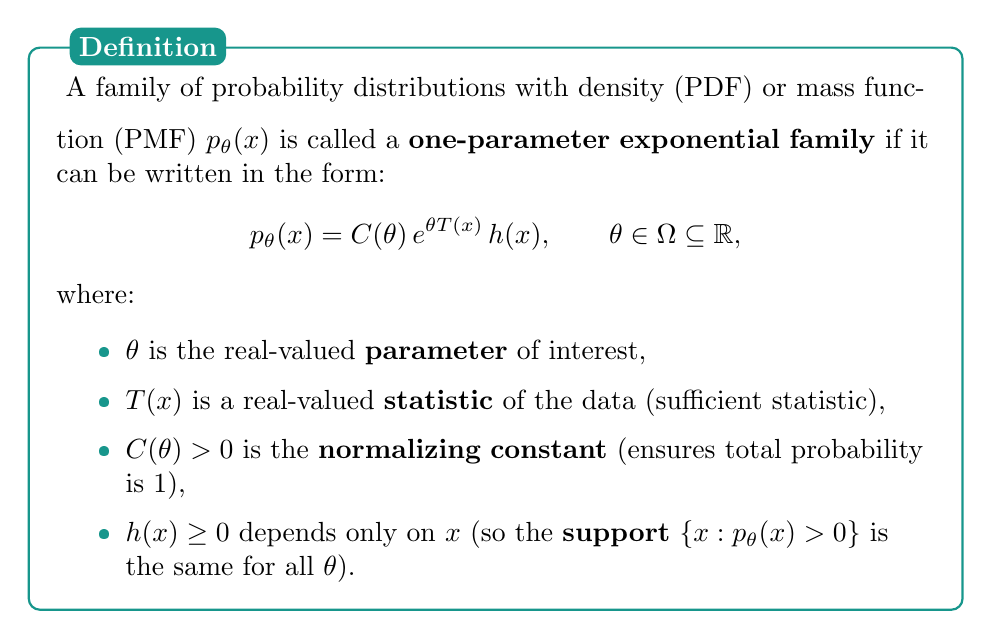
\begin{tikzpicture}
        \node[draw=Teal, thick, rounded corners, inner sep=10pt, text width=0.92\textwidth] (defbox) {
            \vspace*{0.25cm}
            A family of probability distributions with density (PDF) or mass function (PMF) $p_\theta(x)$ is called a \textbf{one-parameter exponential family} if it can be written in the form:
            \[
                p_\theta(x) = C(\theta)\, e^{\theta T(x)}\, h(x), \qquad \theta \in \Omega \subseteq \mathbb{R},
            \]
            where:
            \begin{itemize}
                \setlength\itemsep{2pt}
                \item[\textcolor{Teal}{\textbullet}] $\theta$ is the real-valued \textbf{parameter} of interest,
                \item[\textcolor{Teal}{\textbullet}] $T(x)$ is a real-valued \textbf{statistic} of the data (sufficient statistic),
                \item[\textcolor{Teal}{\textbullet}] $C(\theta) > 0$ is the \textbf{normalizing constant} (ensures total probability is $1$),
                \item[\textcolor{Teal}{\textbullet}] $h(x) \ge 0$ depends only on $x$ (so the \textbf{support} $\{x : p_\theta(x) > 0\}$ is the same for all $\theta$).
            \end{itemize}
        };
        \node[fill=Teal, text=white, rounded corners, right=15pt] at (defbox.north west) {\bfseries Definition};        
    \end{tikzpicture}
\end{frame}

\begin{frame}{One-Parameter Exponential Families}
    \centering
    % Definition Box
    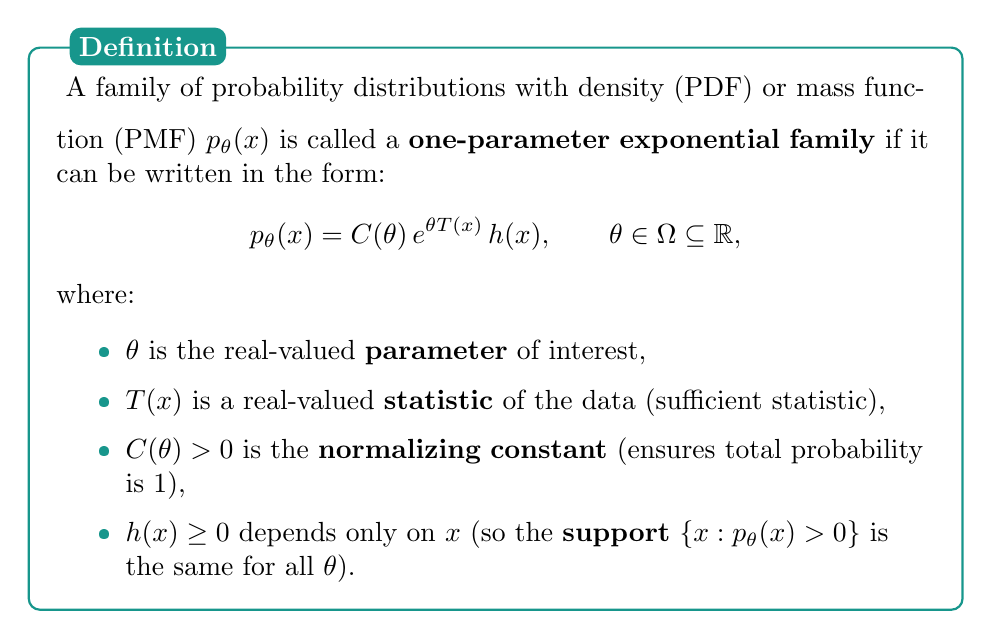
\begin{tikzpicture}
        \node[draw=Teal, thick, rounded corners, inner sep=10pt, text width=0.92\textwidth] (defbox) {
            \vspace*{0.25cm}
            A family of probability distributions with density (PDF) or mass function (PMF) $p_\theta(x)$ is called a \textbf{one-parameter exponential family} if it can be written in the form:
            \[
                p_\theta(x) = C(\theta)\, e^{\theta T(x)}\, h(x), \qquad \theta \in \Omega \subseteq \mathbb{R},
            \]
            where:
            \begin{itemize}
                \setlength\itemsep{2pt}
                \item[\textcolor{Teal}{\textbullet}] $\theta$ is the real-valued \textbf{parameter} of interest,
                \item[\textcolor{Teal}{\textbullet}] $T(x)$ is a real-valued \textbf{statistic} of the data (sufficient statistic),
                \item[\textcolor{Teal}{\textbullet}] $C(\theta) > 0$ is the \textbf{normalizing constant} (ensures total probability is $1$),
                \item[\textcolor{Teal}{\textbullet}] $h(x) \ge 0$ depends only on $x$ (so the \textbf{support} $\{x : p_\theta(x) > 0\}$ is the same for all $\theta$).
            \end{itemize}
        };
        \node[fill=Teal, text=white, rounded corners, right=15pt] at (defbox.north west) {\bfseries Definition};
    \end{tikzpicture}
\end{frame}


% --- Theorem 3.7.1 (1/2) ---
\begin{frame}{Theorem 3.7.1 : UMP Tests for Two-Sided Hypotheses (1/2)}
    
    \lead{Theorem}\\
    \vspace{0.2cm}
    
    \noindent
    {\color{Teal}\vrule width 4pt}%
    \hspace{10pt}%
    \begin{minipage}{\dimexpr\textwidth-14pt\relax}
        \color{Slate}
        Let $X$ have a distribution from a one-parameter exponential family with density $p_\theta(x) = C(\theta)\, e^{\theta T(x)}\, h(x)$. Consider testing the composite null hypothesis $H : \theta \le \theta_1 \text{ or } \theta \ge \theta_2$ ($\theta_1 < \theta_2$) against the alternative $K : \theta_1 < \theta < \theta_2$.
        
        \vspace{0.15cm}
        Then:
        \vspace{0.15cm}
        \begin{itemize}
            \item[{\tikz[baseline=(char.base)]{\node[shape=circle,draw=Teal,inner sep=1pt,text=Teal,font=\scriptsize\bfseries] (char) {i};}}] \lead{Existence \& Structure:} For any level $\alpha \in (0,1)$, there exists a UMP test given by
            \[
                \phi(x) = \begin{cases}
                    1, & \text{when } C_1 < T(x) < C_2 \quad (C_1 \le C_2), \\
                    \gamma_i, & \text{when } T(x) = C_i, \quad i = 1, 2, \\
                    0, & \text{when } T(x) < C_1 \text{ or } T(x) > C_2,
                \end{cases}
            \]
            where $C_1, C_2$ and $\gamma_1, \gamma_2 \in [0,1]$ are determined by $E_{\theta_1}[\phi(X)] = E_{\theta_2}[\phi(X)] = \alpha$.
        \end{itemize}
    \end{minipage}
\end{frame}

% --- Theorem 3.7.1 (2/2) ---
\begin{frame}{Theorem 3.7.1 : UMP Tests for Two-Sided Hypotheses (2/2)}
    
    \lead{Theorem (Continued)}\\
    \vspace{0.2cm}
    
    \noindent
    {\color{Teal}\vrule width 4pt}%
    \hspace{10pt}%
    \begin{minipage}{\dimexpr\textwidth-14pt\relax}
        \color{Slate}
        For the UMP level $\alpha$ test $\phi$ defined in Part (i):
        \vspace{0.2cm}
        \begin{itemize}
            \setlength\itemsep{8pt}
            \item[{\tikz[baseline=(char.base)]{\node[shape=circle,draw=Teal,inner sep=1pt,text=Teal,font=\scriptsize\bfseries] (char) {ii};}}] \lead{Minimization on $H$:} This test \textbf{minimizes} $E_\theta[\phi(X)]$ subject to the boundary condition
            \[
                E_{\theta_1}[\phi(X)] = E_{\theta_2}[\phi(X)] = \alpha
            \]
            for all $\theta < \theta_1$ and all $\theta > \theta_2$.
            
        \end{itemize}
    \end{minipage}
\end{frame}
% --- Proof of Theorem 3.7.1: Step 1 (1/3) ---
\begin{frame}{Proof of Theorem 3.7.1 : Step 1 (1/3)}
    
    \lead{Relaxed Problem \& Interiority Goal}\\
    \vspace{0.2cm}
    
    \color{Slate}
    Fix an arbitrary alternative $\theta' \in (\theta_1, \theta_2)$. We first solve the relaxed problem of maximizing
    \[
        \int_{\mathcal{X}} \phi(x) p_{\theta'}(x)\, d\mu
    \]
    subject to the two boundary constraints
    \[
        \int_{\mathcal{X}} \phi(x) p_{\theta_1}(x)\, d\mu \le \alpha
        \qquad \text{and} \qquad
        \int_{\mathcal{X}} \phi(x) p_{\theta_2}(x)\, d\mu \le \alpha.
    \]
    
    \vspace{0.15cm}
    To apply \textbf{Theorem 3.6.1}, we must verify that $(\alpha, \alpha) \in \operatorname{Int}(M)$, where
    \[
        M \triangleq \left\{ \left(\int_{\mathcal{X}} \phi p_{\theta_1}\, d\mu,\; \int_{\mathcal{X}} \phi p_{\theta_2}\, d\mu\right) \;\middle|\; \phi \in \Phi \right\} \subseteq [0,1]^2.
    \]
    \begin{itemize}
        \item[\textcolor{Teal}{\textbullet}] \textbf{Diagonal Endpoints:} Taking $\phi \equiv 0$ and $\phi \equiv 1$ immediately gives $(0,0) \in M$ and $(1,1) \in M$.
    \end{itemize}
\end{frame}

% --- Proof of Theorem 3.7.1: Step 1 (2/3) ---
\begin{frame}{Proof of Theorem 3.7.1 : Step 1 (2/3)}
    
    \lead{Constructing $\phi_+$ and $\phi_-$ via Neyman--Pearson}\\
    \vspace{0.2cm}
    
    \color{Slate}
    Since $\theta_1 < \theta_2$, we have $P_{\theta_1} \neq P_{\theta_2}$.
    \vspace{0.15cm}
    \begin{itemize}
        \setlength\itemsep{8pt}
        \item[\textcolor{Teal}{\textbullet}] \textbf{Point Strictly Above $(\alpha, \alpha)$:} By the \textbf{Neyman--Pearson Lemma}, there exists a test $\phi_+ \in \Phi$ and $k \ge 0$ with $\displaystyle \int_{\mathcal{X}} \phi_+ p_{\theta_1}\, d\mu = \alpha$ such that
        \[
            \int_{\mathcal{X}} (\phi_+ - \alpha)(p_{\theta_2} - k p_{\theta_1})\, d\mu > 0
            \implies \int_{\mathcal{X}} \phi_+ p_{\theta_2}\, d\mu > \alpha.
        \]
        
        \item[\textcolor{Teal}{\textbullet}] \textbf{Point Strictly Below $(\alpha, \alpha)$:} Applying the same argument at level $1 - \alpha$ yields $\psi \in \Phi$ with
        \[
            \int_{\mathcal{X}} \psi p_{\theta_1}\, d\mu = 1 - \alpha
            \qquad \text{and} \qquad
            \int_{\mathcal{X}} \psi p_{\theta_2}\, d\mu > 1 - \alpha.
        \]
        Setting $\phi_- \triangleq 1 - \psi$ gives $\displaystyle \int_{\mathcal{X}} \phi_- p_{\theta_1}\, d\mu = \alpha$ and $\displaystyle \int_{\mathcal{X}} \phi_- p_{\theta_2}\, d\mu < \alpha$.
    \end{itemize}
\end{frame}

% --- Proof of Theorem 3.7.1: Step 1 (3/3) ---
\begin{frame}{Proof of Theorem 3.7.1 : Step 1 (3/3)}
    
    \lead{Convexity of $M$ \& Invoking Theorem 3.6.1}\\
    \vspace{0.2cm}
    
    \begin{columns}[T, onlytextwidth]
        \begin{column}{0.56\textwidth}
            \color{Slate}
            \begin{itemize}
                \setlength\itemsep{8pt}
                \item[\textcolor{Teal}{\textbullet}] \textbf{Convexity:} Since $M$ is convex and $0 < \alpha < 1$, $(\alpha, \alpha)$ lies strictly inside the quadrilateral formed by $(0,0)$, $(1,1)$, $(\alpha, E_{\theta_2}[\phi_+])$, and $(\alpha, E_{\theta_2}[\phi_-])$.
                
                \item[\textcolor{Teal}{\textbullet}] \textbf{Result:} $(\alpha, \alpha) \in \operatorname{Int}(M)$. By \textbf{Theorem 3.6.1}, there exist an optimal test $\phi^*$ and constants $k_1, k_2 \ge 0$ such that
                \[
                    \phi^*(x) = \begin{cases}
                        1, & p_{\theta'}(x) > k_1 p_{\theta_1}(x) + k_2 p_{\theta_2}(x), \\
                        0, & p_{\theta'}(x) < k_1 p_{\theta_1}(x) + k_2 p_{\theta_2}(x).
                    \end{cases}
                \]
            \end{itemize}
        \end{column}
        
        \begin{column}{0.40\textwidth}
            \centering
            \vspace{0.2cm}
            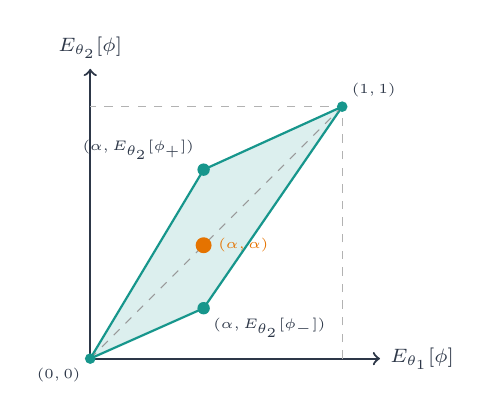
\begin{tikzpicture}[scale=3.2]
                % Axes
                \draw[->, Slate, thick] (0,0) -- (1.15,0) node[right, font=\scriptsize] {$E_{\theta_1}[\phi]$};
                \draw[->, Slate, thick] (0,0) -- (0,1.15) node[above, font=\scriptsize] {$E_{\theta_2}[\phi]$};
                
                % Unit square boundary
                \draw[dashed, black!30] (1,0) -- (1,1) -- (0,1);
                
                % Filled convex quadrilateral inside M
                \fill[Teal!15] (0,0) -- (0.45,0.20) -- (1,1) -- (0.45,0.75) -- cycle;
                \draw[Teal, thick] (0,0) -- (0.45,0.20) -- (1,1) -- (0.45,0.75) -- cycle;
                
                % Diagonal
                \draw[dashed, black!40] (0,0) -- (1,1);
                
                % Points
                \fill[Teal] (0,0) circle (0.6pt) node[below left, font=\tiny, Slate] {$(0,0)$};
                \fill[Teal] (1,1) circle (0.6pt) node[above right, font=\tiny, Slate] {$(1,1)$};
                \fill[Teal] (0.45,0.75) circle (0.7pt) node[above left, font=\tiny, Slate] {$(\alpha, E_{\theta_2}[\phi_+])$};
                \fill[Teal] (0.45,0.20) circle (0.7pt) node[below right, font=\tiny, Slate] {$(\alpha, E_{\theta_2}[\phi_-])$};
                
                % Interior point (alpha, alpha)
                \fill[orange!90!black] (0.45,0.45) circle (0.9pt);
                \node[right, font=\tiny\bfseries, orange!90!black] at (0.47,0.45) {$(\alpha, \alpha)$};
            \end{tikzpicture}
        \end{column}
    \end{columns}
\end{frame}

% --- Proof of Theorem 3.7.1: Step 2 (1/3) ---
\begin{frame}{Proof of Theorem 3.7.1 : Step 2 (1/3)}
    
    \lead{Proving Strict Positivity: $k_1 > 0$ and $k_2 > 0$}\\
    \vspace{0.2cm}
    
    \color{Slate}
    From Step 1, Theorem 3.6.1 gives an optimal test $\phi^*$ and constants $k_1, k_2 \ge 0$ such that
    \[
        \phi^*(x) = \begin{cases}
            1, & \text{if } p_{\theta'}(x) > k_1 p_{\theta_1}(x) + k_2 p_{\theta_2}(x), \\
            0, & \text{if } p_{\theta'}(x) < k_1 p_{\theta_1}(x) + k_2 p_{\theta_2}(x).
        \end{cases}
    \]
    We rule out the three boundary cases where at least one multiplier is zero.
    
    \vspace{0.25cm}
    \begin{itemize}
        \item[\textcolor{Teal}{\textbullet}] \textbf{Case 1: $k_1 = 0$ and $k_2 = 0$.}
        \vspace{0.1cm}
        \begin{itemize}
            \setlength\itemsep{4pt}
            \item The rejection condition reduces to $p_{\theta'}(x) > 0$.
            \item Since all $p_\theta(x) = C(\theta) e^{\theta T(x)} h(x)$ share the same support $\{x : h(x) > 0\}$, this forces $\phi^*(x) = 1$ everywhere $p_{\theta_1}(x) > 0$.
            \item Hence $\displaystyle \int_{\mathcal{X}} \phi^*(x) p_{\theta_1}(x)\, d\mu = 1 > \alpha$, violating the constraint $\mathbb{E}_{\theta_1}[\phi^*] \le \alpha$. \textbf{Contradiction.}
        \end{itemize}
    \end{itemize}
\end{frame}

% --- Proof of Theorem 3.7.1: Step 2 (2/3) ---
\begin{frame}{Proof of Theorem 3.7.1 : Step 2 (2/3)}
    
    \lead{Case 2: $k_1 > 0$ and $k_2 = 0$}\\
    \vspace{0.2cm}
    
    \color{Slate}
    \begin{itemize}
        \setlength\itemsep{6pt}
        \item[\textcolor{Teal}{\textbullet}] The rejection condition simplifies to $p_{\theta'}(x) > k_1 p_{\theta_1}(x)$. Substituting the exponential family density and canceling $h(x) > 0$:
        \[
            C(\theta') e^{\theta' T(x)} > k_1 C(\theta_1) e^{\theta_1 T(x)}
            \iff e^{(\theta' - \theta_1) T(x)} > k_1 \frac{C(\theta_1)}{C(\theta')}.
        \]
        
        \item[\textcolor{Teal}{\textbullet}] Since $\theta_1 < \theta' < \theta_2$, we have $\theta' - \theta_1 > 0$. Taking logarithms yields a \textbf{right-tailed test}:
        \[
            T(x) > C, \qquad \text{where } C = \frac{1}{\theta' - \theta_1} \ln\!\left(k_1 \frac{C(\theta_1)}{C(\theta')}\right).
        \]
        
        \item[\textcolor{Teal}{\textbullet}] Because $k_1 > 0$, complementary slackness forces $\mathbb{E}_{\theta_1}[\phi^*] = \alpha$.
        
        \item[\textcolor{Teal}{\textbullet}] By the \textbf{MLR property}, the power function $\beta_{\phi^*}(\theta)$ of a non-trivial right-tailed test is \textbf{strictly increasing} in $\theta$. Since $\theta_2 > \theta_1$:
        \[
            \mathbb{E}_{\theta_2}[\phi^*] > \mathbb{E}_{\theta_1}[\phi^*] = \alpha,
        \]
        violating $\mathbb{E}_{\theta_2}[\phi^*] \le \alpha$. \textbf{Contradiction.}
    \end{itemize}
\end{frame}

% --- Proof of Theorem 3.7.1: Step 2 (3/3) ---
\begin{frame}{Proof of Theorem 3.7.1 : Step 2 (3/3)}
    
    \lead{Case 3: $k_1 = 0, k_2 > 0$ \& Conclusion}\\
    \vspace{0.2cm}
    
    \color{Slate}
    \begin{itemize}
        \setlength\itemsep{6pt}
        \item[\textcolor{Teal}{\textbullet}] \textbf{Case 3 ($k_1 = 0, k_2 > 0$):} The rejection condition becomes $p_{\theta'}(x) > k_2 p_{\theta_2}(x)$, i.e.,
        \[
            e^{(\theta' - \theta_2) T(x)} > k_2 \frac{C(\theta_2)}{C(\theta')}.
        \]
        Since $\theta' - \theta_2 < 0$, dividing by $(\theta' - \theta_2)$ reverses the inequality, yielding a \textbf{left-tailed test} $T(x) < C$.
        
        \item[\textcolor{Teal}{\textbullet}] Here $k_2 > 0$ forces $\mathbb{E}_{\theta_2}[\phi^*] = \alpha$. By MLR, $\beta_{\phi^*}(\theta)$ is \textbf{strictly decreasing} in $\theta$, so $\theta_1 < \theta_2$ implies
        \[
            \mathbb{E}_{\theta_1}[\phi^*] > \mathbb{E}_{\theta_2}[\phi^*] = \alpha,
        \]
        violating $\mathbb{E}_{\theta_1}[\phi^*] \le \alpha$. \textbf{Contradiction.}
    \end{itemize}
    
    \vspace{0.2cm}
    \noindent
    {\color{Teal}\vrule width 4pt}%
    \hspace{10pt}%
    \begin{minipage}{\dimexpr\textwidth-14pt\relax}
        \textbf{Result of Step 2:} Both multipliers are strictly positive (\textbf{$k_1 > 0$ and $k_2 > 0$}), and both boundary constraints hold with equality:
        \[
            \mathbb{E}_{\theta_1}[\phi^*(X)] = \mathbb{E}_{\theta_2}[\phi^*(X)] = \alpha.
        \]
    \end{minipage}
\end{frame}

% --- Proof of Theorem 3.7.1: Step 3 (1/3) ---
\begin{frame}{Proof of Theorem 3.7.1 : Step 3 (1/3)}
    
    \lead{Rewriting the Optimality Condition}\\
    \vspace{0.2cm}
    
    \color{Slate}
    From Steps 1--2, we have $k_1, k_2 > 0$ and the rejection condition
    \[
        p_{\theta'}(x) > k_1 p_{\theta_1}(x) + k_2 p_{\theta_2}(x).
    \]
    Dividing both sides by $p_{\theta'}(x) = C(\theta') e^{\theta' T(x)} h(x) > 0$ (on the common support $\{x : h(x) > 0\}$) gives
    \[
        1 > a_1 e^{(\theta_1 - \theta') T(x)} + a_2 e^{(\theta_2 - \theta') T(x)},
    \]
    where the constants are strictly positive:
    \[
        a_1 \triangleq k_1 \frac{C(\theta_1)}{C(\theta')} > 0
        \qquad \text{and} \qquad
        a_2 \triangleq k_2 \frac{C(\theta_2)}{C(\theta')} > 0.
    \]
    
    \vspace{0.15cm}
    Define $g(t) \triangleq a_1 e^{(\theta_1 - \theta') t} + a_2 e^{(\theta_2 - \theta') t}$. Then $\phi^*(x) = 1$ when $g(T(x)) < 1$ and $\phi^*(x) = 0$ when $g(T(x)) > 1$.
\end{frame}

% --- Proof of Theorem 3.7.1: Step 3 (2/3) ---
\begin{frame}{Proof of Theorem 3.7.1 : Step 3 (2/3)}
    
    \lead{Shape of the Function $g(t)$}\\
    \vspace{0.2cm}
    
    \color{Slate}
    Recall that $\theta_1 < \theta' < \theta_2$, so $\theta_1 - \theta' < 0$ and $\theta_2 - \theta' > 0$. We examine the calculus of $g(t) = a_1 e^{(\theta_1 - \theta') t} + a_2 e^{(\theta_2 - \theta') t}$:
    
    \vspace{0.15cm}
    \begin{itemize}
        \setlength\itemsep{8pt}
        \item[\textcolor{Teal}{\textbullet}] \textbf{Behavior at $\pm\infty$:} Since $a_1, a_2 > 0$, the first term blows up as $t \to -\infty$ and the second blows up as $t \to +\infty$:
        \[
            \lim_{t \to -\infty} g(t) = +\infty
            \qquad \text{and} \qquad
            \lim_{t \to +\infty} g(t) = +\infty.
        \]
        
        \item[\textcolor{Teal}{\textbullet}] \textbf{Strict Convexity:} Differentiating twice with respect to $t$:
        \[
            g''(t) = a_1 (\theta_1 - \theta')^2 e^{(\theta_1 - \theta') t} + a_2 (\theta_2 - \theta')^2 e^{(\theta_2 - \theta') t} > 0 \qquad \forall t \in \mathbb{R}.
        \]
        Hence $g(t)$ is \textbf{strictly convex} (U-shaped) and attains a unique global minimum.
    \end{itemize}
\end{frame}

% --- Proof of Theorem 3.7.1: Step 3 (3/3) ---
\begin{frame}{Proof of Theorem 3.7.1 : Step 3 (3/3)}
    
    \lead{Deriving the Interval Structure $(C_1, C_2)$}\\
    \vspace{0.2cm}
    
    \begin{columns}[T, onlytextwidth]
        \begin{column}{0.56\textwidth}
            \color{Slate}
            \begin{itemize}
                \setlength\itemsep{6pt}
                \item[\textcolor{Teal}{\textbullet}] Since $\mathbb{E}_{\theta_1}[\phi^*(X)] = \alpha > 0$, the set $\{t : g(t) \le 1\}$ must be non-empty, so $\min_t g(t) \le 1$ (By Contradiction).
                
                \item[\textcolor{Teal}{\textbullet}] By strict convexity, the horizontal line $y = 1$ intersects $g(t)$ at most twice, at $C_1 \le C_2$, with
                \[
                    g(t) < 1 \iff C_1 < t < C_2.
                \]
                
                \item[\textcolor{Teal}{\textbullet}] Thus $\phi^*$ has the exact desired form:
                \[
                    \phi^*(x) = \begin{cases}
                        1, & C_1 < T(x) < C_2, \\
                        \gamma_i, & T(x) = C_i \;\; (i=1,2), \\
                        0, & T(x) < C_1 \text{ or } T(x) > C_2.
                    \end{cases}
                \]
            \end{itemize}
        \end{column}
        
        \begin{column}{0.40\textwidth}
            \centering
            \vspace{0.3cm}
            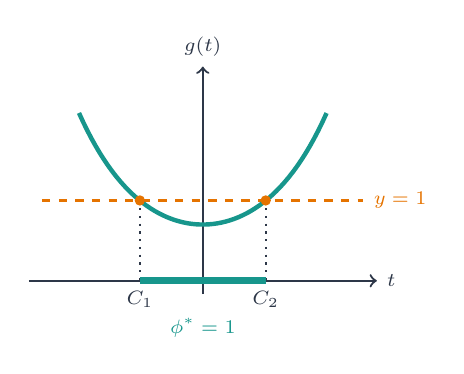
\begin{tikzpicture}[scale=0.85]
                % Axes
                \draw[->, Slate, thick] (-2.6,0) -- (2.6,0) node[right, font=\scriptsize] {$t$};
                \draw[->, Slate, thick] (0,-0.2) -- (0,3.2) node[above, font=\scriptsize] {$g(t)$};
                
                % Horizontal line y = 1
                \draw[dashed, orange!90!black, thick] (-2.4,1.2) -- (2.4,1.2) node[right, font=\scriptsize] {$y = 1$};
                
                % Strictly convex curve g(t) = 0.45*exp(-0.9*t) + 0.45*exp(0.9*t) shifted visually
                \draw[Teal, ultra thick, domain=-1.85:1.85, samples=60] plot (\x, {0.42*exp(-0.95*\x) + 0.42*exp(0.95*\x)});
                
                % Intersection points (approx x = +/- 0.94 where y = 1.2)
                \draw[dotted, Slate, thick] (-0.94,1.2) -- (-0.94,0) node[below, font=\scriptsize] {$C_1$};
                \draw[dotted, Slate, thick] (0.94,1.2) -- (0.94,0) node[below, font=\scriptsize] {$C_2$};
                \fill[orange!90!black] (-0.94,1.2) circle (2.2pt);
                \fill[orange!90!black] (0.94,1.2) circle (2.2pt);
                
                % Highlight rejection interval on axis
                \draw[Teal, line width=2.5pt] (-0.94,0) -- (0.94,0);
                \node[below=10pt, font=\scriptsize\bfseries, Teal] at (0,0) {$\phi^* = 1$};
            \end{tikzpicture}
        \end{column}
    \end{columns}
\end{frame}

% --- Proof of Theorem 3.7.1: Step 4A (1/3) ---
\begin{frame}{Proof of Theorem 3.7.1 : Step 4A (1/3)}
    
    \lead{Uniformity Over All Alternatives $\theta'' \in (\theta_1, \theta_2)$}\\
    \vspace{0.2cm}
    
    \color{Slate}
    We now freeze $\phi^*$ (with cutoffs $C_1 < C_2$ and $\mathbb{E}_{\theta_1}[\phi^*] = \mathbb{E}_{\theta_2}[\phi^*] = \alpha$) and fix an arbitrary alternative $\theta'' \in (\theta_1, \theta_2)$.
    
    \vspace{0.15cm}
    \begin{itemize}
        \setlength\itemsep{6pt}
        \item[\textcolor{Teal}{\textbullet}] \textbf{Goal:} Show $\phi^*$ maximizes $\mathbb{E}_{\theta''}[\phi(X)]$ among all tests satisfying $\mathbb{E}_{\theta_1}[\phi] \le \alpha$ and $\mathbb{E}_{\theta_2}[\phi] \le \alpha$.
        
        \item[\textcolor{Teal}{\textbullet}] \textbf{Strategy (Theorem 3.6.1 — Sufficiency, Inequality Version):} It suffices to find constants $k_1'', k_2'' > 0$ such that
        \[p_{\theta''}(x) > k_1'' p_{\theta_1}(x) + k_2'' p_{\theta_2}(x) \iff C_1 < T(x) < C_2.\]
        
        \item[\textcolor{Teal}{\textbullet}] Dividing by $p_{\theta''}(x) > 0$ and setting $a_i \triangleq k_i'' \dfrac{C(\theta_i)}{C(\theta'')}$, we define
        \[g_{\theta''}(t) \triangleq a_1 e^{(\theta_1 - \theta'') t} + a_2 e^{(\theta_2 - \theta'') t}.\]
        We need $a_1, a_2 > 0$ such that $g_{\theta''}(C_1) = 1$ and $g_{\theta''}(C_2) = 1$.
    \end{itemize}
\end{frame}

% --- Proof of Theorem 3.7.1: Step 4A (2/3) ---
\begin{frame}{Proof of Theorem 3.7.1 : Step 4A (2/3)}
    
    \lead{Reverse-Engineering Positive Multipliers $a_1, a_2 > 0$}\\
    \vspace{0.2cm}
    
    \color{Slate}
    For $i \in \{1, 2\}$, define $u_i \triangleq e^{(\theta_1 - \theta'') C_i}$ and $v_i \triangleq e^{(\theta_2 - \theta'') C_i}$. The boundary equations $g_{\theta''}(C_1) = 1$ and $g_{\theta''}(C_2) = 1$ form a $2 \times 2$ linear system:
    \[
        \begin{cases}
            u_1 a_1 + v_1 a_2 = 1, \\
            u_2 a_1 + v_2 a_2 = 1.
        \end{cases}
    \]
    
    \vspace{0.1cm}
    Since $\theta_1 - \theta'' < 0 < \theta_2 - \theta''$ and $C_1 < C_2$, we have the strict orderings:
    \[
        u_1 > u_2 > 0
        \qquad \text{and} \qquad
        0 < v_1 < v_2.
    \]
    Therefore, the determinant is strictly positive: $D = u_1 v_2 - u_2 v_1 > 0$. By Cramer's Rule:
    \[
        a_1 = \frac{v_2 - v_1}{D} > 0
        \qquad \text{and} \qquad
        a_2 = \frac{u_1 - u_2}{D} > 0.
    \]
\end{frame}

% --- Proof of Theorem 3.7.1: Step 4A (3/3) ---
\begin{frame}{Proof of Theorem 3.7.1 : Step 4A (3/3)}
    
    \lead{Verifying Optimality for $\theta''$}\\
    \vspace{0.2cm}
    
    \color{Slate}
    \begin{itemize}
        \setlength\itemsep{6pt}
        \item[\textcolor{Teal}{\textbullet}] Since $a_1, a_2 > 0$, the corresponding multipliers satisfy
        \[
            k_1'' = a_1 \frac{C(\theta'')}{C(\theta_1)} > 0
            \qquad \text{and} \qquad
            k_2'' = a_2 \frac{C(\theta'')}{C(\theta_2)} > 0.
        \]
        
        \item[\textcolor{Teal}{\textbullet}] Just as in Step 3, $a_1, a_2 > 0$ implies $g_{\theta''}''(t) > 0$ for all $t \in \mathbb{R}$, so $g_{\theta''}(t)$ is \textbf{strictly convex}.
        
        \item[\textcolor{Teal}{\textbullet}] Because $g_{\theta''}(C_1) = g_{\theta''}(C_2) = 1$, strict convexity guarantees
        \[
            g_{\theta''}(t) < 1 \iff C_1 < t < C_2
            \qquad \text{and} \qquad
            g_{\theta''}(t) > 1 \iff t < C_1 \text{ or } t > C_2.
        \]
    \end{itemize}
    
    \vspace{0.15cm}
    \noindent
    {\color{Teal}\vrule width 4pt}%
    \hspace{10pt}%
    \begin{minipage}{\dimexpr\textwidth-14pt\relax}
        \textbf{Conclusion of Step 4A:} By Theorem 3.6.1 (Sufficiency), $\phi^*$ maximizes $\mathbb{E}_{\theta''}[\phi(X)]$ for \textbf{every} $\theta'' \in (\theta_1, \theta_2)$ among all tests with $\mathbb{E}_{\theta_1}[\phi] \le \alpha$ and $\mathbb{E}_{\theta_2}[\phi] \le \alpha$.
    \end{minipage}
\end{frame}

% --- Proof of Theorem 3.7.1: Step 4B (1/3) ---
\begin{frame}{Proof of Theorem 3.7.1 : Step 4B (1/3)}
    
    \lead{Part (ii): Minimization on $H$ ($\theta_0 < \theta_1$ or $\theta_0 > \theta_2$)}\\
    \vspace{0.2cm}
    
    \color{Slate}
    Fix any $\theta_0 < \theta_1$ (the case $\theta_0 > \theta_2$ is symmetric). We prove that $\phi^*$ \textbf{minimizes} $\mathbb{E}_{\theta_0}[\phi(X)]$ among all tests satisfying $\mathbb{E}_{\theta_1}[\phi] = \mathbb{E}_{\theta_2}[\phi] = \alpha$.
    
    \vspace{0.15cm}
    \begin{itemize}
        \setlength\itemsep{6pt}
        \item[\textcolor{Teal}{\textbullet}] \textbf{Flip to Maximization:} For any test $\phi$, define $\psi \triangleq 1 - \phi$. Minimizing $\mathbb{E}_{\theta_0}[\phi]$ is equivalent to \textbf{maximizing} $\mathbb{E}_{\theta_0}[\psi]$ subject to
        \[
            \mathbb{E}_{\theta_1}[\psi(X)] = 1 - \alpha
            \qquad \text{and} \qquad
            \mathbb{E}_{\theta_2}[\psi(X)] = 1 - \alpha.
        \]
        
        \item[\textcolor{Teal}{\textbullet}] \textbf{Structure of $\psi^* \triangleq 1 - \phi^*$:}
        \[
            \psi^*(x) = \begin{cases}
                1, & \text{if } T(x) < C_1 \text{ or } T(x) > C_2 \quad \text{(outer tails)}, \\
                0, & \text{if } C_1 < T(x) < C_2 \quad \text{(middle interval)}.
            \end{cases}
        \]
    \end{itemize}
\end{frame}

% --- Proof of Theorem 3.7.1: Step 4B (2/3) ---
\begin{frame}{Proof of Theorem 3.7.1 : Step 4B (2/3)}
    
    \lead{Applying Theorem 3.6.1 (Sufficiency --- Equality Version)}\\
    \vspace{0.2cm}
    
    \color{Slate}
    Because the constraints are \textbf{equalities}, Theorem 3.6.1 only requires $k_1', k_2' \in \mathbb{R}$ (signs unrestricted). Dividing $p_{\theta_0} - k_1' p_{\theta_1} - k_2' p_{\theta_2}$ by $p_{\theta_0}(x) > 0$ and setting $b_i \triangleq k_i' \dfrac{C(\theta_i)}{C(\theta_0)}$, define
    \[
        r(t) \triangleq 1 - b_1 e^{(\theta_1 - \theta_0) t} - b_2 e^{(\theta_2 - \theta_0) t}.
    \]
    
    \begin{itemize}
        \setlength\itemsep{6pt}
        \item[\textcolor{Teal}{\textbullet}] \textbf{Matching the Cutoffs:} Solving $r(C_1) = 0$ and $r(C_2) = 0$ yields a unique pair $(b_1, b_2)$ since $\theta_1 \neq \theta_2$ and $C_1 \neq C_2$.
        
        \item[\textcolor{Teal}{\textbullet}] \textbf{Counting Roots via Rolle's Theorem:} Setting $r'(t) = 0$ gives
        \[
            e^{(\theta_2 - \theta_1) t} = -\frac{b_1(\theta_1 - \theta_0)}{b_2(\theta_2 - \theta_0)},
        \]
        which has \textbf{at most one} solution. By Rolle's Theorem, $r(t)$ has at most two roots ($C_1$ and $C_2$) and \textbf{must change sign} at both.
    \end{itemize}
\end{frame}

% --- Proof of Theorem 3.7.1: Step 4B (3/3) ---
\begin{frame}{Proof of Theorem 3.7.1 : Step 4B (3/3)}
    
    \lead{Sign Trace \& Completing the Proof of Parts (i) and (ii)}\\
    \vspace{0.2cm}
    
    \color{Slate}
    \begin{itemize}
        \setlength\itemsep{6pt}
        \item[\textcolor{Teal}{\textbullet}] \textbf{Sign at $-\infty$:} Since $\theta_0 < \theta_1 < \theta_2$, both exponents $(\theta_1 - \theta_0)$ and $(\theta_2 - \theta_0)$ are positive, so
        \[
            \lim_{t \to -\infty} r(t) = 1 - 0 - 0 = 1 > 0.
        \]
        
        \item[\textcolor{Teal}{\textbullet}] \textbf{Exact Match with $\psi^*$:} Crossing $0$ at $C_1$ and $C_2$ gives $r(t) > 0$ on $(-\infty, C_1) \cup (C_2, \infty)$ and $r(t) < 0$ on $(C_1, C_2)$. By Theorem 3.6.1, $\psi^*$ maximizes $\mathbb{E}_{\theta_0}[\psi]$, so \textbf{$\phi^*$ minimizes $\mathbb{E}_{\theta_0}[\phi]$}. \textbf{(Proves Part (ii).)}
    \end{itemize}
    
    \vspace{0.15cm}
    \noindent
    {\color{Teal}\vrule width 4pt}%
    \hspace{10pt}%
    \begin{minipage}{\dimexpr\textwidth-14pt\relax}
        \textbf{Completing Part (i):} Comparing $\phi^*$ with the constant test $\phi_c \equiv \alpha$ (which also satisfies $\mathbb{E}_{\theta_1}[\phi_c] = \mathbb{E}_{\theta_2}[\phi_c] = \alpha$) gives
        \[
            \mathbb{E}_{\theta_0}[\phi^*(X)] \le \mathbb{E}_{\theta_0}[\phi_c(X)] = \alpha \qquad \forall \theta_0 \in H.
        \]
        Hence $\phi^*$ is a valid level $\alpha$ test on $H$, and by Step 4A it is \textbf{UMP} for $H$ vs.\ $K$. \hfill $\square$
    \end{minipage}
\end{frame}

% --- Final Slide: Thank You ---
\begin{frame}[plain]
    % Left vertical accent bar (matching transition slide)
    \begin{tikzpicture}[remember picture, overlay]
        \fill[Teal] (current page.north west) rectangle ([xshift=0.55cm]current page.south west);
    \end{tikzpicture}

    \centering
    \vspace*{1.6cm}

    {\Huge\bfseries\color{Teal} Thank You!\par}

    \vspace{0.35cm}

    % Subtle accent divider
    
\begin{tikzpicture}
        \draw[Teal, line width=2pt] (-2.2,0) -- (1.2,0);
        \draw[orange!90!black, line width=2pt] (1.2,0) -- (2.2,0);
    \end{tikzpicture}

    \vspace{0.45cm}

    {\Large\color{Slate} Questions \& Discussion\par}

    \vspace{1.2cm}

    {\normalsize\bfseries\color{Slate} Abhishek Jha\par}
    \vspace{0.1cm}
    {\small\color{black!65} Two-Sided Hypothesis Testing (Lehmann \& Romano, Sections 3.6--3.7)\par}
    \vspace{0.05cm}
    {\small\color{black!55} University of Luxembourg \textbullet\ November 24, 2026\par}
\end{frame}

\end{document}